
\begin{quote}
    "Mathematics is the art of reducing any problem to linear algebra" - William Stein
\end{quote}


Linear algebra is one of the foundational concepts in mathematics, and is essential to properly understanding multivariable calculus.

We will begin by studying certain properties of $\R^n$, and we will see how $\R^n$ and its properties can be generalized to vector spaces.  We will then study how vectors spaces can be compared to each other, through linear maps.

%\fixthis{more intro}

\section{An introduction to $\R^n$}

\begin{definition}
Given a positive integer $n$, \textbf{$n$-dimensional Euclidean space} (denoted $\R^n$) is the set of all ordered $n$-tuples of real numbers.  That is,
$$\R^n := \{(x_1, \cdots ,x_n) \ | \ x_i \in \R\}$$
\end{definition}

\begin{example}
    We are familiar with $\R^1$ (often described as the real line $\R$),
    
    \begin{center}
        \begin{tikzpicture}[x=1cm, y=1cm, z=-0.6cm, scale=0.5]
    % Axes
    \draw [<->] (-4,0,0) -- (4,0,0) node [right] {};

    % Ticks
        \foreach \i in {-3,-2, -1, 0, 1,2,3}
    {
    \draw (\i,-0.1,0) -- ++ (0,0.2,0);
    }

\end{tikzpicture}
    \end{center}
    
    as well as $\R^2$ (often described as the Euclidean plane), which has the $x$ and $y$ axes.
    
    \begin{center}
                \begin{center}\begin{tikzpicture}[scale=.65]
    \pgfmathsetmacro{\entrya}{3}
\pgfmathsetmacro{\entryb}{2}
\clip (-3,-3) rectangle (3,3);
 % Axes
    \draw [<->] (-3,0) -- (3,0) node [below left] {$x$};
    \draw [<->] (0,-3) -- (0,3) node [below right] {$y$};

\end{tikzpicture}
        \end{center}
        \end{center}
    
\end{example}

\begin{example}
    $\R^3$ is often described as Euclidean space, and has 3 axes (denoted the $x$, $y$, and $z$ axes).
    
    \begin{center}
            \begin{tikzpicture}[x=1cm, y=1cm, z=-0.6cm, scale=0.5]
            \pgfmathsetmacro{\cubex}{3}
\pgfmathsetmacro{\cubey}{2.5}
\pgfmathsetmacro{\cubez}{3.14}
    % Axes
    \draw [<->] (-4,0,0) -- (4,0,0) node [right] {$y$};
    \draw [<->] (0,-4,0) -- (0,4,0) node [left] {$z$};
    \draw [<->] (0,0,-4) -- (0,0,4) node [left] {$x$};

    % Ticks
        \foreach \i in {-3,-2, -1, 0, 1,2,3}
    {
    \draw (-0.1,\i,0) -- ++ (0.2,0,0);
    \draw (\i,-0.1,0) -- ++ (0,0.2,0);
    \draw (-0.1,0,\i) -- ++ (0.2,0,0);
    }

\end{tikzpicture}
        \end{center}
    
\end{example}


We can study and understand $n$-dimensional Euclidean space in many different ways by imposing different \textit{structures} on the set $\R^n$.  For example, we might wish to consider $\R^n$ geometrically (more precisely, as a topological space).

Thinking geometrically, an element $\bm{x} = (x_1, \cdots ,x_n) \in \R^n$ can be thought of as describing \textit{coordinates} that tell us precisely where $\bm{x}$ is located inside of $\R^n$.  In this framework, we will call elements of $\R^n$ points.

\begin{definition}
A \textbf{point in $\R^n$} (often denoted $\bm{x} \in \R^n$) is an element of $\R^n$, considered as a topological space.  That is, 
$$\bm{x} = (x_1, x_2, \cdots, x_n)$$

We say that $x_1$ is the \textbf{first coordinate}, $x_2$ is the second coordinate, and so on, until $x_n$ (which is the $n$-th coordinate).
\end{definition}

\begin{example}
    The point $O = (0, 0, \cdots, 0) \in \R^n$ is called the \textbf{origin} (in $\R^n$). 
\end{example}

\begin{example}
We can also consider the point $P = (\pi, 3, 2.5) \in \R^3$.  

The first coordinate tells us that along the $x$-axis, we are $\pi$ units in the positive direction from the origin; the second coordinate tells us we are 3 units in the positive direction along the $y$-axis, and the third coordinate tells us we are 2.5 units in the positive direction along the $z$-axis.

We can visualize $P$ by drawing a box such that one corner is at the origin, the edges are aligned with the axes in $\R^3$, and the dimensions of the box correspond with the coordinates.  $P$ is then the corner of the box that is furthest from the origin.

 \begin{center}
            \begin{tikzpicture}[x=1cm, y=1cm, z=-0.6cm, scale=0.5]
            \pgfmathsetmacro{\cubex}{3}
\pgfmathsetmacro{\cubey}{2.5}
\pgfmathsetmacro{\cubez}{3.14}
    % Axes
    \draw [->] (0,0,0) -- (4,0,0) node [right] {$y$};
    \draw [->] (0,0,0) -- (0,4,0) node [left] {$z$};
    \draw [->] (0,0,0) -- (0,0,4) node [left] {$x$};

    \draw[megreen,dashed, thick] (0,0,0) -- (\cubex,0,0);
    \draw[megreen,dashed, thick] (0,\cubey,0) -- (\cubex,\cubey,0);
    \draw[megreen,dashed, thick] (0,0,\cubez) -- (\cubex,0,\cubez);
    \draw[megreen,dashed, thick] (0,\cubey,\cubez) -- (\cubex,\cubey,\cubez);
    
    \draw[UCLAblue,dashed, thick] (0,0,0) -- (0,\cubey,0);
    \draw[UCLAblue,dashed, thick] (\cubex,0,0) -- (\cubex,\cubey,0);
    \draw[UCLAblue,dashed, thick] (0,0,\cubez) -- (0,\cubey,\cubez);
    \draw[UCLAblue,dashed, thick] (\cubex,0,\cubez) -- (\cubex,\cubey,\cubez);
    
    \draw[red,dashed, thick] (0,0,0) -- (0,0,\cubez);
    \draw[red,dashed, thick] (\cubex,0,0) -- (\cubex,0,\cubez);
    \draw[red,dashed, thick] (0,\cubey,0) -- (0,\cubey,\cubez);
    \draw[red,dashed, thick] (\cubex,\cubey,0) -- (\cubex,\cubey,\cubez);
    
    \filldraw[black] (\cubex,\cubey,\cubez) circle (2pt) node[anchor=west]{P};
    % % Vectors
    % \draw [->, thick] (0,0,0) -- (2,2,0);
    % \draw [->, thick] (0,0,0) -- (2,0,1);
    % Ticks
        \foreach \i in {1,2,3}
    {
    \draw (-0.1,\i,0) -- ++ (0.2,0,0);
    \draw (\i,-0.1,0) -- ++ (0,0.2,0);
    \draw (-0.1,0,\i) -- ++ (0.2,0,0);
    }

\end{tikzpicture}
        \end{center}
\end{example}


On the other hand, we are not required to think of $\R^n$ in this way.  Indeed, the structures that we impose on $\R^n$ should reflect how we want to think.

For example, we can instead think of an element $\bm{v} = (v_1, \cdots, v_n) \in \R^n$ not as describing coordinates, but rather, as describing \textit{\textbf{displacement}}.  In other words, given a starting point $P$ and an ending point $Q$, we can measure the \textit{change} in each coordinate.  In this framework, we will call elements of $\R^n$ vectors:

\begin{definition}
A \textbf{vector in $\R^n$}\define{vector in $\R^n$} (often denoted $\bm{v} \in \R^n$) is an element of $\R^n$, considered as a vector space.  That is,
$$\bm{v} = \langle v_1, \cdots, v_n \rangle$$

We say that $v_1$ is the \textbf{first component}\define{vector component}, $v_2$ is the second component, and so on, until $v_n$ (which is the $n$-th component).
\end{definition}



\begin{example}
Suppose that you started at the point $P = (3, 0, \pi) \in \R^3$, and ended up at the point $Q = (4, 3, e) \in \R^3$.  Then your total displacement along the $x$-axis is $4-3=1$ unit; $3-0=3$ units along the $y$-axis; and $e-\pi$ units along the $z$-axis.  Then your total displacement can be described as a vector
$$\bm{PQ} = \langle 1, 3, e-\pi \rangle \in \R^3$$

We can visualize the vector $\bm{PQ}$ as an arrow in $\R^3$, starting at $P$ and ending at $Q$:

 \begin{center}
            \begin{tikzpicture}[x=1cm, y=1cm, z=-0.6cm, scale=0.5]
\pgfmathsetmacro{\cubex}{0}
\pgfmathsetmacro{\cubey}{3.14}
\pgfmathsetmacro{\cubez}{3}
\pgfmathsetmacro{\cubexx}{3}
\pgfmathsetmacro{\cubeyy}{2.72}
\pgfmathsetmacro{\cubezz}{4}
    % Axes
    \draw [->] (0,0,0) -- (4,0,0) node [right] {$y$};
    \draw [->] (0,0,0) -- (0,4,0) node [left] {$z$};
    \draw [->] (0,0,0) -- (0,0,4) node [left] {$x$};
    
    \draw[UCLAblue, thick, ->] (\cubex,\cubey,\cubez) -- (\cubexx,\cubeyy,\cubezz);
    
    \filldraw[black] (\cubex,\cubey,\cubez) circle (2pt) node[anchor=west]{P};
    \filldraw[black] (\cubexx,\cubeyy,\cubezz) circle (2pt) node[anchor=west]{Q};
    % % Vectors
    % \draw [->, thick] (0,0,0) -- (2,2,0);
    % \draw [->, thick] (0,0,0) -- (2,0,1);
    % Ticks
        \foreach \i in {1,2,3}
    {
    \draw (-0.1,\i,0) -- ++ (0.2,0,0);
    \draw (\i,-0.1,0) -- ++ (0,0.2,0);
    \draw (-0.1,0,\i) -- ++ (0.2,0,0);
    }

\end{tikzpicture}
        \end{center}

We say that the terminal point $Q$ is the \textbf{head}\define{head} of the vector $\bm{PQ}$, and that the initial point $P$ is the \textbf{tail}\define{tail} of the vector $\bm{PQ}$

\end{example}


Given a vector $\bm{PQ}$, we can recover information about the relationship between the points $P$ and $Q$.  For example, we can calculate the distance between two points $P$ and $Q$ in $\R^3$ by iterating the Pythagorean theorem twice:

\begin{example}
    The distance between $P = (1,1,1)$ and $Q = (\pi, 3, 2.5)$  is $\sqrt{(\pi-1)^2+ (3-1)^2 + (2.5-1)^2}$
    
    \begin{center}
            \begin{tikzpicture}[x=1cm, y=1cm, z=-0.6cm, scale=0.5]
\pgfmathsetmacro{\cubex}{3}
\pgfmathsetmacro{\cubey}{4}
\pgfmathsetmacro{\cubez}{3.14}
    % Axes
    \draw [->] (0,0,0) -- (4,0,0) node [right] {$y$};
    \draw [->] (0,0,0) -- (0,4,0) node [left] {$z$};
    \draw [->] (0,0,0) -- (0,0,4) node [left] {$x$};
    
    \draw[red, thick] (1,1,1) -- (1,1,\cubez);
    \draw[megreen, thick] (1,1,\cubez) -- (\cubex,1,\cubez);
    \draw[UCLAblue, thick] (\cubex,1,\cubez) -- (\cubex,\cubey,\cubez);
    
    \draw[mepink,dashed, thick](1,1,1) -- (\cubex,1,\cubez);
    \draw[UTorange,dashed, thick] (1,1,1) -- (\cubex,\cubey,\cubez);
    
    \filldraw[black] (\cubex,1,\cubez) circle (2pt) node[anchor=west]{$(\pi, 1, 2.5)$};
    \filldraw[black] (\cubex,\cubey,\cubez) circle (2pt) node[anchor=west]{P};
    \filldraw[black] (1,1,1) circle (2pt) node[anchor=east]{O};
    % % Vectors
    % \draw [->, thick] (0,0,0) -- (2,2,0);
    % \draw [->, thick] (0,0,0) -- (2,0,1);
    % Ticks
        \foreach \i in {1,2,3}
    {
    \draw (-0.1,\i,0) -- ++ (0.2,0,0);
    \draw (\i,-0.1,0) -- ++ (0,0.2,0);
    \draw (-0.1,0,\i) -- ++ (0.2,0,0);
    }

\end{tikzpicture}
        \end{center}

Observe that the points $P$, $(\pi, 1, 1)$, and $(\pi, 1, 2.5)$ form a right triangle, whose hypotenuse has length $\sqrt{(\pi-1)^2+(2.5-1)^2}$. Similarly, the points $P$, $(\pi, 1, 2.5)$, and $Q$ also form a right triangle, where the length of the hypotenuse is precisely the distance between $P$ and $Q$.

    
\end{example}

Observe that the distance between $P = (1,1,1)$ and $Q = (\pi, 3, 2.5)$  is precisely the square root of the sum of the squares of the components of the vector $\bm{PQ}$. That is, if we write the components of $\bm{PQ} = \langle \pi-1, 2, 1.5 \rangle = \langle v_1, v_2, v_3 \rangle$, then the distance between $P$ and $Q$ is $$\sqrt{v_1^2 + v_2^2 + v_3^2}$$  

This observation generalizes to $\R^n$, as we would need to iterate the Pythagorean theorem $n-1$ times.  If we consider two points $P = (x_1, \cdots, x_n)$ and $Q = (y_1, \cdots, y_n)$,
and write the components of the vector $\bm{PQ} = \langle x_1-y_1, \cdots, x_n-y_n \rangle = \langle v_1, \cdots, v_n \rangle$, we again find that the distance between $P$ and $Q$ is $$\sqrt{v_1^2 + \cdots + v_n^2}$$

Thus, we should give this quantity a name:

    \begin{definition}
    Given a vector $\bm{v} = \langle v_1, \cdots, v_n \rangle$, its \textbf{magnitude}\define{magnitude} is given by $$||\bm{v}|| = \sqrt{\sum_{i=1}^n v_i^2}$$
    \end{definition}

    \begin{proposition}
        The distance between two points $P = (x_1, \cdots, x_n)$ and $Q = (y_1, \cdots, y_n)$ is precisely $||\bm{PQ}||$.
    \end{proposition}
    
    \begin{example}
    The vector $\bm{PQ} = \langle 1, 3, e-\pi \rangle \in \R^3$ has magnitude $$||\bm{PQ}|| = \sqrt{1^2+3^2 + (e-\pi)^2}$$
    \end{example}
    

    \begin{definition}
    A \textbf{unit vector}\define{unit vector} in $\R^n$ is a vector $\bm{u} \in \R^n$ such that $||\bm{u}|| = 1$.
    \end{definition}

    \begin{example}
        In $\R^3$, there are special unit vectors, called the \textbf{standard basis vectors} of $\R^3$:
        
        $$\bm{i} = \langle 1, 0, 0 \rangle$$
        $$\bm{j} = \langle 0, 1, 0 \rangle$$
        $$\bm{k} = \langle 0, 0, 1 \rangle$$
        
            \begin{center}
            \begin{tikzpicture}[x=1cm, y=1cm, z=-0.6cm, scale=0.5]

    % Axes
    \draw [->] (0,0,0) -- (4,0,0) node [right] {$y$};
    \draw [->] (0,0,0) -- (0,4,0) node [left] {$z$};
    \draw [->] (0,0,0) -- (0,0,4) node [left] {$x$};
    
    \draw[red, ultra thick, ->] (0,0,0) -- (0,0,1) node [left] {$i$};
    \draw[megreen,ultra thick, ->] (0,0,0) -- (0,1,0) node [right]{$k$};
    \draw[UCLAblue,ultra thick, ->] (0,0,0) -- (1,0,0) node [below] {$j$};
    
    % % Vectors
    % \draw [->, thick] (0,0,0) -- (2,2,0);
    % \draw [->, thick] (0,0,0) -- (2,0,1);
    % Ticks
        \foreach \i in {1,2,3}
    {
    \draw (-0.1,\i,0) -- ++ (0.2,0,0);
    \draw (\i,-0.1,0) -- ++ (0,0.2,0);
    \draw (-0.1,0,\i) -- ++ (0.2,0,0);
    }

\end{tikzpicture}
        \end{center}
        
    \end{example}

    \begin{example}
    The vector $\bm{e_{PQ}} = \left\langle \frac{1}{\sqrt{(e-\pi)^2+10}}, \frac{3}{\sqrt{(e-\pi)^2+10}}, \frac{e-\pi}{\sqrt{(e-\pi)^2+10}} \right\rangle \in \R^3$ is a unit vector.
    \end{example}







\begin{motivating}
What are the differences between the points perspective and the vectors perspective?
\end{motivating}

Though the two perspectives might seem similar, there are important differences:

For example, from the points perspective, we should think of elements in $\R^n$ as being analogous to \textit{locations} on a map.  It \textbf{doesn't make sense} to add the location of Los Angeles, California (say, coordinates with latitude $34^\circ$ N, longitude $118^\circ$ W) to the location of Austin, Texas (say, coordinates $30^\circ$ N, $98^\circ$ W).

On the other hand, from the vectors perspective, we should think of elements in $\R^n$ as being analogous to displacements.  In this case, let us consider two displacements:
The displacement from Los Angeles to Austin means travelling $4^\circ$ south, and travelling $20^\circ$ east. Similarly, the displacement from Austin to New York City (coordinates $41^\circ$ N, $74^\circ$ W) means travelling $11^\circ$ north, and travelling $24^\circ$ east.

It \textbf{does make sense} to add these two displacements together, which entails travelling a total of $7^\circ$ north, and $44^\circ$ east.  Observe that the result of this addition is the \textbf{total displacement} from Los Angeles to New York City (travelling $7^\circ$ north, and $44^\circ$ east).

We can formulate this in terms of vectors as follows:

\begin{definition}[Vector addition]

\define{vector addition} Given two vectors $\bm{u} = \langle u_1, \cdots, u_n \rangle$, $\bm{v} = \langle v_1, \cdots, v_n \rangle$, we can add  two vectors together to form the sum $\bm{u+v} \in \R^n$.  In terms of components,
$$\bm{u+v} = \langle u_1+v_1, \cdots, u_n+v_n \rangle$$

\end{definition}

\begin{example}
    There is a nice geometric picture that accompanies vector addition:  Given two vectors $\bm{PQ}$ and $\bm{QR}$, then the sum of these two vectors is the vector $\bm{PR}$ (that is, the vector with tail $P$, and head $R$)
    
    \begin{center}
            \begin{tikzpicture}[scale=0.7]
            \pgfmathsetmacro{\cubex}{2}
            \pgfmathsetmacro{\cubey}{3}

    
    
    \draw[red, thick, -Latex] (0,0) -- (\cubex,1) node[midway,below right] {$\bm{PQ}$};
    \draw[megreen, thick, -Latex] (\cubex,1) -- (\cubex,\cubey) node[midway, right] {$\bm{QR}$};
    \draw[UCLAblue, thick, -Latex] (0,0) -- (\cubex,\cubey) node[midway,above left] {$\bm{PR}$};
    
    
    \filldraw[black] (0,0) circle (2pt) node[anchor=east]{P};
    \filldraw[black] (\cubex,1) circle (2pt) node[anchor=west]{Q};
    \filldraw[black] (\cubex,\cubey) circle (2pt) node[anchor=west]{R};
    
    \end{tikzpicture}
        \end{center}
        
    That is, we add vectors "tip to tail".
\end{example}


\begin{proposition}
    Vector addition is commutative.  That is, the vectors $\bm{u+v}$ and $\bm{v+u}$ are the same vector.
\end{proposition}

\begin{example}
    This follows immediately from the definition in terms of components.  However, there is a nice geometric picture that accompanies this property:
    
    
    \begin{center}
            \begin{tikzpicture}scale=0.5]
            \pgfmathsetmacro{\cubex}{2}
            \pgfmathsetmacro{\cubey}{3}

    
    
    \draw[red, thick, -Latex] (0,0) -- (\cubex,1) node[midway,below right] {$\bm{u}$};
    \draw[megreen, thick, -Latex] (\cubex,1) -- (\cubex,\cubey) node[midway, right] {$\bm{v}$};
    \draw[UCLAblue, thick, -Latex] (0,0) -- (\cubex,\cubey) node[midway,above left] {$\bm{u+v}$};
    \draw[megreen, thick, -Latex] (0,0) -- (0,\cubey-1) node[midway,left] {$\bm{v}$};
    \draw[red, thick, -Latex] (0, \cubey-1) -- (\cubex,\cubey) node[midway,left] {$\bm{u}$};
    
    
    
    \end{tikzpicture}
        \end{center}
        
    That is, if we move our vectors freely, the $\bm{u+v}$ is the diagonal of the parallelogram spanned by $\bm{u}$ and $\bm{v}$.
\end{example}

Let us be more precise about moving vectors freely:  we can combine the points perspective with the vector perspective.  Using our previous analogies, it makes sense to add the add the \textit{displacement} from Los Angeles to Austin to the \textit{location} New York City.  

We should interpret this as saying to start at the coordinates $41^\circ$ N, $74^\circ$ W, and to then travel  $4^\circ$  south, and $20^\circ$ east.  The end result is a \textbf{location} with coordinates $37^\circ$ N, $54^\circ$ W (somewhere in the middle of the  Atlantic Ocean!).

We can formulate this in terms of vectors as follows:

\begin{definition}\label{pointvector}
In terms of coordinates, given a point $P = (x_1, \cdots, x_n) \in \R^n$, and a vector $\bm{v} = \langle v_1, \cdots, v_n \rangle \in \R^n$, then we can define the \textbf{point} $P + \bm{v}$ to be the point with coordinates $$P + \bm{v} = (x_1 + v_1 , \cdots, x_n + v_n)$$
\end{definition}

Informally, the point  $P + \bm{v}$ is the tail of the vector that starts at $P$, and travels along the length of $\bm{v}$. We can also make this mathematically precise through vector addition:

\begin{definition}
A \textbf{position vector}\define{position vector} in $\R^n$ is a vector whose tail (or initial point) is the origin.

If the head of the position vector is the point $P$, then we often denote the position vector as the vector $\bm{OP}$.
\end{definition}


\begin{proposition}
Given a point $P \in \R^n$, and a vector $\bm{v}\in \R^n$, the point $P + \bm{v}$ has the same coordinates as the head (or terminal point) of the vector $\bm{OP} + \bm{v}$.    
\end{proposition}


We are now able to describe various vectors at different locations in $\R^n$.  We have seen cases where two vectors indeed start and end at the same point, but in definition \ref{pointvector}, we now see that it is possible for "the same vector" to have different starting points. This leads us to the following question:

\begin{motivating}
When are two vectors the same?
\end{motivating}

We first must define what we mean for two vectors to be the same:


\begin{definition}

    A vector $\bm{w} = \bm{AB}$ is said to be \textbf{equivalent}\define{equivalent vector} to a vector $\bm{v} = \bm{PQ}$ if the terminal point $B$ is the same as the point $A + \bm{v}$
    
    We sometimes also say that $\bm{w}$ is a \textbf{translation} of $\bm{v}$.
    
\end{definition}

\begin{example}
    Suppose that we have a vector $\bm{v} = PQ \in \R^n$, and suppose that the components of $\bm{v}$ are $\bm{v} = \langle v_1, \cdots, v_n \rangle$.
    
    Consider the point $P = (v_1, \cdots, v_n)$.  Then $\bm{v}$ is equivalent to the position vector $\bm{OP}$, which starts at the origin $O$, and ends at the point $P$.
\end{example}


The example above is the key idea of the proof of the following proposition:

\begin{proposition}
    Consider the points $A, B, P, Q \in \R^n$.  The vectors $\bm{AB}$ and $\bm{PQ}$ are equivalent if and only if they have the same components.
\end{proposition}











We now turn to a second way to distinguish vectors:



\begin{definition}\label{scalar}
A \textbf{scalar}\define{scalar} (often denoted $\lambda \in \R$) is an element of the field of real numbers, $\R$.
\end{definition}

    \begin{definition}
    Given a vector $\bm{v} = \langle v_1, \cdots , v_n\rangle \in \R^n$ and a scalar $\lambda \in \R$, the \textbf{scalar multiple}\define{scalar multiple}  $\lambda \bm{v}$ is the vector $$\lambda \bm{v} = \langle \lambda v_1, \cdots, \lambda v_n \rangle$$
    
    That is, we multiply $\lambda$ with each component.
  \end{definition}


We can interpret scalar multiples geometrically through the following calculation:

\begin{proposition}
  The magnitude of a scalar multiple $\lambda \bm{v}$ is the same as the magnitude of $\bm{v}$ times the absolute value of $\lambda$.  That is, $$||\lambda\bm{v}|| = |\lambda|(||\bm{v}||)$$
\end{proposition}

 \begin{example}
 This tells us that scalar multiplication changes the magnitude of a vector (that is, it \textit{scales} it by a factor of $|\lambda|$).  
 
        \begin{center}
            \begin{tikzpicture}scale=0.5]
            \pgfmathsetmacro{\cubex}{1}
            \pgfmathsetmacro{\cubey}{3}

    
    
    \draw[red, thick, -Latex] (-1,0) -- (-1+\cubex,\cubex) node[midway, left] {$\bm{v}$};
    \draw[megreen, thick, -Latex] (1,0) -- (2*\cubex+1,2*\cubex) node[midway, right] {$2\bm{v}$};
    \draw[UCLAblue, thick, -Latex] (0,0) -- (-\cubex,-\cubex) node[midway, right] {$-\bm{v}$};
    
    
    
    \end{tikzpicture}
        \end{center}
    \end{example}


\begin{definition}
Two vectors $\bm{v}, \bm{w} \in \R^n$ are said to be \textbf{parallel}\define{parallel vectors} if they are scalar multiples of each other.  That is, there exists a scalar $\lambda \in \R$ such that $$\bm{v} = \lambda \bm{w}$$
\end{definition}

\begin{example}

    Consider the points $P = (3, -2, 1)$ and $Q = (2, -1, 1)$  in $\R^3$, and consider the vectors $\bm{u} = \langle -1, 1, 0 \rangle$, $\bm{v} = \langle -2, 2, 0 \rangle$, $\bm{w} = \langle 1, -1, 0 \rangle$,  $\bm{a} = \langle 1, -1, 1 \rangle$.
    
    \begin{itemize}
        \item The vector $\bm{PQ}$ is equivalent to $\bm{u}$.
        \item The vector $\bm{PQ}$ is parallel to $\bm{v}$, with $\lambda = 2$.
        \item The vector $\bm{PQ}$ is parallel to $\bm{w}$, with $\lambda = -1$.
        \item The vector $\bm{PQ}$ is \textbf{not} parallel to $\bm{a}$. That is, there is no $\lambda$ such that $\bm{PQ} = \lambda \bm{a}$.
        
        If such a $\lambda$, existed, that would require that the equations $-1 = \lambda 1$ and $0 = \lambda 1$ to both be true.  But that would be a contradiction, since $\lambda$ cannot be both $-1$ and $0$.
    \end{itemize}
    
\end{example}


Parallel vectors are so named because they give rise to parallel lines.  See definition \ref{linesinrn} in the exercises to learn how we describe lines in $\R^n$, and exercise \ref{problem:parametrizationsparallel}.

Observe that in the example above, we saw that two vectors can be parallel, yet point in different directions.  We can make this idea precise:

    \begin{definition}
    Given a non-zero vector $\bm{v} \in \R^n$, its \textbf{direction vector}\define{direction vector} $\bm{e_v}$ is the unit vector such that 
    $$||\bm{v}||\bm{e_v} = \bm{v}$$
    \end{definition}

Note that we used the word "the" in the definition above - in order for this definition to make sense, we should make sure to prove that the direction vectors is \textit{unique}.

\begin{proposition}
    Given a non-zero vector $\bm{v} \in \R^n$, its \textbf{direction vector}\define{direction vector} $\bm{e_v}$ is unique.  That is, $$\bm{e_v} = \frac{1}{||\bm{v}||}\bm{v}$$
\end{proposition}

Thus, we can now algebraically explain the difference between the vectors $\bm{PQ}$ and $\bm{QP}$:

\begin{definition}
Suppose that the vector $\bm{w}$ is parallel to $\bm{v}$, with $\bm{v} = \lambda \bm{w}$.  If $\lambda > 0$, then we say $\bm{w}$ has the \textbf{same direction} as $\bm{v}$.  If $\lambda < 0$, then $\bm{w}$ has the \textbf{opposite direction} as $\bm{v}$.
\end{definition}



\begin{proposition}
    Two vectors are equivalent if and only if they have the same magnitude and the same direction vector.
\end{proposition}


In other words, if two vectors have different magnitudes, then they must be different vectors.  Similarly, if two vectors have different direction vectors, then they must be different vectors.

To summarize, we have learned the following:

    \begin{example}
    
    A vector in $\R^n$ is determined equivalently by:
    
    \begin{enumerate}
        \item an initial point and a terminal point. $$v = \bm{PQ}$$
        \item its components. $$\bm{v} = \langle x_1, \cdots, x_n \rangle$$
        \item a direction and magnitude. $$\bm{v} = ||\bm{v}||\bm{e_v}$$
    \end{enumerate}
    \end{example}










% Thinking of elements in $\R^n$ as displacements has some advantages that will naturally leads us to the study of vector spaces and linear algebra.






\subsection{Exercises}

\begin{problem}{pointsandvectors}
Explain the relationship between points and vectors.

More concretely, given a point in $\R^n$, is there a natural way to obtain a vector in $\R^n$?  Conversely, given a vector in $\R^n$, is there a natural way to obtain a point in $\R^n$?
\end{problem}

\begin{answer}{pointsandvectors}
Position vectors.
\end{answer}

\begin{problem}{componentsunit}
    Sketch and find the components of the unit position vector in $\R^2$ that makes an angle of $30$ degrees counterclockwise from the positive $x$-axis.
    
\end{problem}

\begin{problem}{sketchequiv}
    Sketch and find the components of the unit position vector in $\R^2$  that makes an angle of $30$ degrees counterclockwise from the negative $x$-axis.
    
    \begin{subproblems}
    \item Is this vector equivalent to the vector in exercise \ref{problem:componentsunit}?
    \item Is this vector parallel to the vector in exercise \ref{problem:componentsunit}?
    \end{subproblems}
    
\end{problem}

\begin{problem}{componentsangle}
    Find the components of the unit position vector in $\R^2$  that makes an angle of $\theta$ degrees counterclockwise from the negative $x$-axis.
\end{problem}

\begin{problem}{parallelvectors}
    Are these vectors parallel to the vector $\bm{v} = \langle 2, -1, 1 \rangle$?  Are they equivalent?
    
    \begin{subproblems}
    \item $\bm{PQ}$, where $P = (1,1,0)$, and $Q = (3, 0, 1)$.
    \item $\bm{QP}$, where $P = (1,1,0)$, and $Q = (3, 0, 1)$.
    \item $\bm{AB}$, where $A = (1,1,0)$, and $B = (5, -1, 2)$.
    \item $\bm{PQ} + 2\bm{AB}$, where $\bm{PQ}$ and $\bm{AB}$ are as above.
    \item $\bm{PQ} + 2\langle 1, 0 ,0 \rangle$, where $\bm{PQ}$ is as above.
    \end{subproblems}
\end{problem}

\begin{problem}{subtractvectors}
    Let $\bm{u} = \langle 1, 1, 0 \rangle$, and let $\bm{v} = \langle 0, 0, 1 \rangle$. 
    
    \begin{subproblems}
    \item Compute $\bm{u-v}$.
    \item Sketch $\bm{u}$, $\bm{v}$, and $\bm{u-v}$.
    \item In general, what is the relationship between  $\bm{u-v}$ and  $\bm{v-u}$?
    \end{subproblems}
\end{problem}

\begin{problem}{parallelogram}
    Given four points, $A$, $B$, $C$, and $D$ in $\R^3$, we obtain a quadrilateral $ABCD$.  If $ABCD$ is a parallelogram, and the coordinates of the corners are $A = (1,0,1)$, $B = (3,3,2)$, and $C = (2,4, 5)$, then what are the coordinates of $D$?
    
    (\textbf{Hint:} Recall that $ABCD$ is given by a line from $A$ to $B$ to $C$ to $D$, and then back to $A$.  Use vectors to solve this problem!).
\end{problem}

\begin{problem}{parallelogramdiagonals}
    Consider the parallelogram $ABCD$.  Prove that the diagonals $BC$ and $AD$ intersect each other at their midpoints.
    
    (\textbf{Hint}: Describe the diagonals as vectors).
\end{problem}


In the following exercises, we will describe lines in $\R^n$.
    
    \begin{definition}\label{linesinrn}
    The line $\mathscr{L}$ in $\R^n$, passing through the point $P = (x_1, \cdots x_n)$, in the direction of the vector $\bm{v} = \langle v_1,  \cdots v_n \rangle$, can be described by the vector-valued function $\bm{r}(t) : \R \to \R^n$ defined by $$\bm{r}(t) = \bm{r_0} + t\bm{v}$$
    
    where $\bm{r_0}$ is the vector $\bm{r_0} = \bm{OP} = \langle x_1, \cdots x_n\rangle$.
    
    We call $\bm{r}(t)$ the \textbf{vector parametrization of} $\mathscr{L}$.
    
    \end{definition}

    Observe that by definition, the vector $\bm{r}(t)$ is a position vector for all $t$.  The tips of these position vectors are precisely the points on the line $\mathscr{L}$.

\begin{problem}{linesinr2}
    
    Recall that we can describe a line in $\R^2$ as the set of points $L = \{(x,y) \ | \ y = mx + b\}$.  Find a vector parametrization of the line $L$.
    
    \begin{subproblems}
    \item What is the relationship between the constant $b$ and the vector $\bm{r_0}$?
    \item What is the relationship between the slope $m$ and the direction vector $\bm{v}$?
    \end{subproblems}
    
\end{problem}

\begin{problem}{line2points}
    Find the vector parametrization of the line that passes through the points $P = (1,0,2)$ and $Q = (2,5,-1)$.
\end{problem}

\begin{problem}{linequniqueness}
    Given a point $P$ and a direction vector $\bm{v}$, is the vector parametrization $\bm{r}(t) = \bm{r_0} + t\bm{v}$ of a line $\mathscr{L}$ unique? 
    
    \begin{subproblems}
    \item Is there a vector parametrization of $\mathscr{L}$ using the same direction vector $\bm{v}$ but a different starting point $Q$?  If so, find the coordinates of a possible $Q$.
    \item Is there a vector parametrization of $\mathscr{L}$ using the same starting point $P$, but a different direction vector, $\bm{w}$?  If so, find the components of a possible $\bm{w}$.
    \item Is there a vector parametrization of $\mathscr{L}$ using a different direction vector $\bm{w}$ and a different starting point $Q$?  If so, find a possible $Q$ and $\bm{w}$.
    \end{subproblems}

    
\end{problem}

\begin{problem}{parametrizationsparallel}
    Suppose that $\bm{r_1}(t) = \bm{r_0} + t\bm{v}$ and $\bm{r_2}(s) = \bm{r_0} + s\bm{w}$ are two parametrizations of the same line.  What is the relationship between $\bm{v}$ and $\bm{w}$?
\end{problem}

\begin{problem}{parametrizationpoints}
    When are $\bm{r_1}(t) = \bm{OP} + t\bm{v}$ and $\bm{r_2}(s) = \bm{OQ} + s\bm{v}$ are two parametrizations of the same line?
\end{problem}

\begin{definition}
We say that two lines $\bm{r_1}(t)$ and $\bm{r_2}(s)$ \textbf{intersect} if there is a point $P$ lying on both lines. 
\end{definition}



\begin{problem}{intersect1}
    Determine whether the following two lines intersect.  If they do, find the common point of intersection.
    $$\bm{r_1}(t) =   \langle3,2,6\rangle + t\langle1,0,-1\rangle$$
    $$\bm{r_2}(s) =   \langle4,12,24\rangle + s\langle-1,10,20\rangle$$
    
    (\textbf{Hint:}  If a point lies on both lines, then that point must satisfy both equations).
\end{problem}

\begin{problem}{intersect2}
    Determine whether the following two lines intersect.  If they do, find the common point of intersection.
    $$\bm{r_1}(t) =   \langle3,2,6\rangle + t\langle1,0,-1\rangle$$
    $$\bm{r_2}(s) =   \langle4,5,1\rangle + s\langle-1,3,3\rangle$$
\end{problem}

\begin{problem}{intersectvscollidelines}
    Suppose that you have two lines with parametrizations $\bm{r_1}(t)$ and $\bm{r_2}(s)$, respectively.  What is the difference between solving the vector equation $\bm{r_1}(t) = \bm{r_2}(s)$ versus solving the vector equation $\bm{r_1}(t) = \bm{r_2}(t)$?
\end{problem}

\begin{definition}
    We say that two distinct lines are \textbf{skew}\define{skew lines}, if they do not intersect each other, and they are not parallel to each other.
    \end{definition}

\begin{problem}{skewlines}
    
    Write down parametrizations of two distinct lines that are skew to each other.  
    
\end{problem}


\section{Vector spaces}

\begin{motivating}
How can we generalize and abstract these properties of $\R^n$?
\end{motivating}

In these lecture notes, we will only study vector spaces whose field of scalars is $\R$ - that is, we are only considering \textit{real} vector spaces\footnote{That is, scalars must be elements of the field $\R$ (as in definition \ref{scalar}).  In other classes, such as linear algebra, you will see that we can generalize by replacing the field $\R$ with any other field $\mathbb{F}$, and a lot of the theory of vector spaces and linear algebra still work over an arbitrary field $\mathbb{F}$.}.  So in these notes we will omit the adjective real and simply refer to them as vector spaces.

    \begin{definition}\label{vspaceaxioms}
    A \textbf{vector space}\define{vector space} $V$ is a set with a distinguished element $\bm{0} \in V$, together with two operations, $+ : V \times V \to V$, and $\cdot : \R \times V \to V$ satisfying the following axioms for all $\bm{u}, \bm{v}, \bm{w} \in V$, and for all $\lambda, \alpha \in \R$.
    
    
     \begin{enumerate}[label=(\roman*)]
        \item $\bm{u} + (\bm{v} + \bm{w}) = (\bm{u} + \bm{v}) + \bm{w} $ (Additive associativity)
        \item $\bm{v} + \bm{0} = \bm{0} + \bm{v} = \bm{v}$ (Additive identity)
        \item For all $\bm{v} \in V$, there exists $\bm{w} \in V$ such that $\bm{v} + \bm{w} = \bm{0}$ (Additive inverse)
        \item $\bm{u} + \bm{v} = \bm{v} + \bm{u}$ (Additive commutativity)
        \item $\lambda (\alpha \bm{v}) = (\lambda\alpha)\bm{v}$ (Scalar associativity)
        \item $1\bm{v} = \bm{v}$ (Scalar identity)
        \item $(\lambda+\alpha)\bm{u} = \lambda\bm{u} +  \alpha\bm{u}$ (Distribution over scalar addition)
        \item $\lambda(\bm{u} + \bm{v}) = \lambda\bm{u} + \lambda\bm{v}$ (Distribution over vector addition)
    \end{enumerate}
    
    The elements of $V$ are called vectors, and elements of $\R$ are called scalars\footnote{see footnote 1}.
    \end{definition}
    
    
When faced with an abstract definition like this, it's especially important to first find a few concrete examples to keep in mind.  Luckily, from our discussion in the previous section, we have in fact checked most of these axioms:
    
    
    \begin{example}
    \vspace{-1em}
    \begin{theorem}
    $\R^n$ is a vector space.
    \end{theorem}
    \end{example}
    
    $\R^n$ is the prototypical example of a vector space\footnote{In fact, in exercise \ref{problem:isotoRn}, you can show that any \textbf{finite dimensional} vector space is isomorphic to $\R^n$.}.  What this means is that whenever you are are trying to determine whether or not something is true about vector spaces, you should try to see if it is true for $\R^n$.  Then, you should try to translate the proof in the $\R^n$ case to the general case, purely using the axioms and properties of abstract vector spaces.
    
    However, you should also be careful not to trick yourself into thinking that every vector space behaves like $\R^n$!  Below is an example of a vector space that is quite different from $\R^n$.  You will verify the axioms in exercise \ref{problem:functionvspace}.
    
    \begin{example}
    \vspace{-1em}
    \begin{theorem}\label{functionsvspace}
    The set $\mathscr{F}(\R)$ of functions $f : \R \to \R$ is a vector space with pointwise addition and pointwise scalar multiplication.  $$(f + g)(x) := f(x) + g(x) \ \qquad \ (\lambda f)(x) := \lambda (f(x))$$
    \end{theorem}
    
    \end{example}

    With these examples in mind, we can now look back at the axioms of a vector space (definition \ref{vspaceaxioms}) and see \textit{why} these axioms are important.

    Axioms $(i)$ through $(iv)$ describe how to \textit{add} vectors using the operation $+ : V \times V \to V$.  From previous experiences with addition, we should require that $+$ should be $(i)$ associative and $(iv)$ commutative.  Moreover, we also require that the zero vector $\bm{0} \in V$ should behave the way that $0 \in \R$ does, with regards to $(ii)$ adding zero, as well as $(iii)$ the existence of additive inverses (e.g. negative numbers in $\R$).

    Axioms $(v)$ through $(vii)$ describe how to \textit{scalar multiply} vectors using the operation $\cdot : \R \times V \to V$.  The intuition for these axioms comes from our knowledge of multiplication for real numbers, which is $(v)$ associative and $(vii)$ distributes over addition of real numbers.  Moreover, the element $1 \in \R$ is the \textit{multiplicative identity} - that is, for any element $a \in \R$, we have that $1(a) = a$.  This property of $1\in \R$ is mirrored in axiom $(vi)$.

    \begin{example}
    \textbf{Warning:} It is important to note, however, that scalar multiplication is \textbf{not} multiplication of vectors.  Indeed, scalar multiplication is a function $\R \times V \to V$.  That is, its input is precisely one scalar and one vector, and whose output is a vector.  You will compare this to multiplication in exercise \ref{problemm:scalarmultvsmult}.
    
    In Section \ref{operations}, we will discuss operations whose inputs are two vectors, and whose output is a vector.
    \end{example}
    
    \subsection{Vector subspaces}
    
    Let us now turn to other examples of vector spaces.
    
    \begin{example}
    Consider the set $$W = \{(x, 0, 0) \in \R^3 \}$$
    
    The first observation to make is that $W$ is a subset of $\R^3$ - that is, every element of $W$ is also contained inside of $\R^3$.  
    
    
    Now, if we take any two elements in $(x_1,0,0), (x_2,0,0) \in W$, we can then add them together as elements of the vector space $\R^3$ to get the vector $(x_1 + x_2, 0,0) \in \R^3$.  Observe that the sum $(x_1 + x_2, 0,0)$ is still an element of $W$ - thus the vector addition in $\R^3$ naturally defines a vector addition on $W$.
    
    Furthermore, if we take an element $(x_1,0,0) \in W$ and a scalar $\lambda \in \R$, we can again treat $(x_1,0,0)$ as an element in $\R^3$, and form the scalar multiple $\lambda((x_1,0,0)) = (\lambda x_1,0,0)$.  Once again, the scalar multiple $\lambda((x_1,0,0))$ is still an element of $W$ - thus the scalar multiplication in $\R^3$ naturally defines a scalar multiplication on $W$.
    
    Thus, we have shown that if we define vector addition and scalar multiplication on $W$ as coming from $\R^3$, it then follows that $W$ satisfies the axioms a vector space.
    \end{example}

    We can now give a name to this phenomenon of a subset of a vector space turning out to be a vector space:
    
    \begin{definition}
    A nonempty subset $W$ of a vector space $V$, is a \textbf{vector subspace}\define{vector subspace} of $V$ if for all $v, w \in W$ and for all $\lambda \in \R$, 
    
    \begin{enumerate}[label=(\roman*)]
        \item $\bm{v} + \bm{w} \in W$ (closure under addition)
        \item $\lambda (\bm{v}) \in W $ (closure under scalar multiplication)
    \end{enumerate}
    
    \end{definition}
    
    Again, to keep ourselves from thinking only in terms of $\R^n$, here is another vector subspace example:
    
    \begin{example}
    \vspace{-1em}
    \begin{theorem}\label{continuousfunctionsvspace}
    The set of $\mathscr{C}(\R)$ of \textit{continuous} functions $f : \R \to \R$ is a vector space with pointwise addition and pointwise scalar multiplication.  $$(f + g)(x) := f(x) + g(x) \ \qquad \ (\lambda f)(x) := \lambda (f(x))$$
    \end{theorem}
    
    \begin{theorem}
    $\mathscr{C}(\R)$ is a subspace of $\mathscr{F}(\R)$.
    \end{theorem}
    
    \end{example}
    
    \textbf{Warning:} It is not true that every subset of a vector space is a vector space.  For a sophisticated example, see  exercise \ref{sumto1}.  For a more immediate example, consider the following:
    
    \begin{example}
    The set of two elements $A = \{(1,0), (0,1)\}$ is a subset of $\R^2$, but is not a vector subspace of $\R^2$, as it fails to be closed under both addition and scalar multiplication.
    \end{example}
    
    In fact, we can generalize this example:
    
    \begin{example}
    \vspace{-1em}
    \begin{proposition}
    If $A$ is a finite set of elements in a vector space contains a non-zero vector, then $A$ cannot be a vector subspace\footnote{Remember, we are considering only real vector spaces in these notes.}.  
    \end{proposition}
    \end{example}
    
    \begin{proof}
    One proof, using vector addition, is as follows:  Suppose that $A$ be a finite set of elements in a vector space with cardinality $|A|=n$, and suppose that $\bm{a} \in A$ is a non-zero vector.  Then consider the sums $\sum_{i=1}^j\bm{a}$ for $1 \leq j \leq n+1$.  Since $\bm{a}$ is non-zero, we have described $n+1$ different vectors, and so at least one of the sums $\sum_{i=1}^j\bm{a}$ cannot be contained in $A$.  Thus $A$ cannot be a vector subspace.  
    
    A variation on this proof can be phrased using scalar multiplication: Let $W$ be a vector subspace of $V$, and let $\bm{w} \in W$ be a non-zero vector.  Then since vector subspaces are closed under scalar multiplication, $W$ contains $\lambda \bm{w}$ for all $\lambda \in \R$.  Moreover, since $\bm{w}$ is non-zero, we have shown that $W$ must have at least as many elements as $\R$.  In other words, we have described an (uncountably) infinite number of elements in $W$, and so any finite set of vectors in a vector space containing a non-zero vector cannot be a vector subspace.
        
    \end{proof}
    

    To phrase this in another way, we have proved that a vector subspace with finitely many elements must be the \textbf{zero} vector space (see exercise \ref{problem:zerovspace}).  However, one might wonder if we can fix this example in some way:

    \begin{motivating}
      Given a (finite) set of elements $A$ in a vector space $V$, can we produce a vector subspace?  Even better, can we produce the \textbf{smallest} vector space containing $A$ (that is, without including any extraneous vectors)?
    \end{motivating}
    
    We see from our observations above to construct the smallest vector space containing $A$, we must first include all scalar multiples of elements in $A$.  Once we have done so, we then need to include any possible sum of scalar multiples.  This is called a \textbf{linear combination}:
    
    \begin{definition}
    Let $V$ be a vector space.  A \textbf{linear combination}\define{linear combination} of vectors $\bm{v_1}, \cdots, \bm{v_k} \in V$ is a vector of the form 
    $$\lambda_1\bm{v_1} + \cdots + \lambda_k\bm{v_k}$$ where the $\lambda_i$ are scalars.
    \end{definition}
    
    Thus, we now have a candidate set for the smallest vector space containing $A$:  the set of all linear combinations of vectors in $A$.
    
    \begin{definition}
    Let $V$ be a vector space, and let $A$ be a subset of vectors in $V$.  The set of all linear combinations of vectors in $A$ is called the \textbf{span} of A, and is written
    $$\textnormal{span}(A)$$
     
\end{definition}
    
    We first must prove that $\textnormal{span}(A)$ is a vector subspace:
    
    \begin{theorem}
    Let $V$ be a vector space, and let $A = \{\bm{v_1}, \cdots, \bm{v_n}\}$ be a set of vectors in $V$.  Then $\textnormal{span}\{\bm{v_1}, \cdots, \bm{v_k}\}$ is a vector subspace of $V$.
    \end{theorem}
    
    \begin{proof}
    We will first prove that $\textnormal{span}\{\bm{v_1}, \cdots, \bm{v_k}\}$ is closed under addition.  Let $\bm{w_1}, \bm{w_2} \in \textnormal{span}\{\bm{v_1}, \cdots, \bm{v_k}\}$.  Then by definition, $$\bm{w_1} = \lambda_1\bm{v_1} + \cdots + \lambda_k\bm{v_k} \qquad \textnormal{and} \qquad \bm{w_2} = \alpha_1\bm{v_1} + \cdots + \alpha_k\bm{v_k}$$
    
    Then by the vector space axioms, $$\bm{w_1} + \bm{w_2} = (\lambda_1+\alpha_1)\bm{v_1} + \cdots + (\lambda_k+\alpha_k)\bm{v_k},$$ Hence $\bm{w_1} + \bm{w_2} \in \textnormal{span}\{\bm{v_1}, \cdots, \bm{v_k}\}$.
    
    We now prove it is closed under scalar multiplication.  Suppose $\lambda$ is an arbitrary scalar.  Then by the vector space axioms, $$\lambda \bm{w_1} = (\lambda\lambda_1)\bm{v_1} + \cdots + (\lambda\lambda_k)\bm{v_k},$$ Hence  $\lambda\bm{w_1} \in \textnormal{span}\{\bm{v_1}, \cdots, \bm{v_k}\}$.
    \end{proof}
    
    \begin{example}
    \begin{proposition}
        Fix a vector $\bm{v} \in V$.  Then $$\textnormal{span}\{\bm{v}\} = \{ \lambda \bm{v} \ | \ \lambda \in \R\}$$
    \end{proposition}
    
    \begin{proof}
    By definition, $\{ \lambda \bm{v} \ | \ \lambda \in \R\} \subseteq \textnormal{span}\{\bm{v}\}$.  On the other hand, since there is only one element in the set $\{\bm{v}\}$, the sum of any elements in $\{\bm{v}\}$ is again a scalar multiple of $\bm{v}$.  Thus we have that $\{ \lambda \bm{v} \ | \ \lambda \in \R\} \supseteq \textnormal{span}\{\bm{v}\}$.
    \end{proof}
    
    
    For example, if $\bm{v}$ is a non-zero element in $\R^n$, then by definition, $\textnormal{span}\{\bm{v}\}$ is a line passing through the origin.
    \end{example}
    
    \begin{example}
    Let $A = \{\langle 1,0 \rangle, \langle 0,1\rangle \}$ be a subset of $\R^2$.  Then $\textnormal{span}(A) = \R^2$.
    
    \begin{proof}
    By definition, $\textnormal{span}(A) \subseteq \R^2$.  On the other hand, pick an arbitrary element $\langle x, y \rangle$ in $\R^2$. We see from the axioms that $x\langle 1,0 \rangle + y\langle 0,1 \rangle = \langle x, y \rangle$.  Thus $\textnormal{span}(A) \supseteq \R^2$.
    \end{proof}
    \end{example}
    
    
    We can now prove that $\textnormal{span}(A)$ is the \textbf{smallest} vector subspace containing $A$.  
    
    \begin{theorem}
    Let $V$ be a vector space, and let $A = \{\bm{v_1}, \cdots, \bm{v_n}\}$ be a set of vectors in $V$.  Suppose $W$ is a vector subspace containing $A$.  Then $W$ contains $\textnormal{span}(A)$.
    \end{theorem}
    
    \begin{proof}
    
    \fixthis{proof}
    \end{proof}
    
    \subsection{Bases}
    
    We have figured out how to construct a vector subspace $\textnormal{span}(A)$ from a given subset $A$.  One natural question to ask is the converse:
    
    \begin{motivating}
     Given a vector subspace $W$, can we construct a subset $B$ such that $W = \textnormal{span}(B)$?  Moreover, is it possible to find a smallest such subset $B$?  
    \end{motivating}
    
    Let us first consider an example:
    
    \begin{example}
    Consider the vector subspace $$W = \{(x, y, 0) \in \R^3 \}$$
    We can write $W$ as the span of several different subsets:
    \begin{enumerate}[label=(\roman*)]
        \item $W= \textnormal{span}\{\langle 1,0,0\rangle, \langle 0,1,0\rangle\}$
        \item $W= \textnormal{span}\{\langle 1,0,0\rangle, \langle 0,1,0\rangle, \langle 2,0,0\rangle\}$
        \item $W= \textnormal{span}\{\langle 1,0,0\rangle, \langle 0,1,0\rangle,\langle 1,1,0\rangle\}$
        \item $W= \textnormal{span}\{\langle 1,0,0\rangle, \langle 0,1,0\rangle, \langle 0, 0, 0\rangle\}$
        \item $W= \textnormal{span}\{\langle 1,0,0\rangle, \langle 0,2,0\rangle\}$
        \item $W= \textnormal{span}\{\langle 1,1,0\rangle, \langle 1,2,0\rangle\}$
    \end{enumerate}
    
    \end{example}
    
    From this collection of examples, we can make a few observations.   Firstly, observe that the sets in examples $(ii)$ to $(iv)$ all contain the set in example $(i)$, yet they all span the subspace $W$.  What this means is that in terms of linear combinations, examples $(ii)$ to $(iv)$ contain extraneous information:
    \begin{itemize}
        \item example $(ii)$ contains two vectors that are scalar multiples of each other;
        \item example $(iii)$ contains a vector that is a linear combination of the other two vectors;
        \item example $(iv)$ also contains a vector that is a linear combination of the other two vectors (see exercise \ref{problem:zerolineardependent}).
    \end{itemize}

    We can make this idea of ``extraneous information" rigorous with the following definition:
    
     \begin{definition}
    A set of vectors $A \subset V$ is said to be \textbf{linearly dependent}\define{linearly dependent} if for every nonempty finite subset of vectors $\{\bm{v_1}, \cdots, \bm{v_k}\} \subset A$, there exist scalars $a_i$, \underline{not all zero}, such that $$a_1\bm{v_1} + \cdots + a_k\bm{v_k} = 0$$ Otherwise, the set $A$ is said to be \textbf{linearly independent}\define{linearly independent}.
    \end{definition}
    
    This condition is precisely the same as our linear combination criterion as discussed above. 
    
    \begin{proposition}
     A set of vectors $A \subset V$ is linearly dependent if and only if one of the vectors is a linear combination of the others.
    \end{proposition}
    
    In some sense, the notion of linear independence gives us a partial answer to finding a ``smallest subset" that spans $W$:
    
    \begin{definition}
    An \underline{ordered} set of vectors $\mathcal{B} \subset V$ is said to be a \textbf{basis}\define{basis} of $V$ if 
     \begin{itemize}
        \item $\textnormal{span}(\mathcal{B}) = V$, and 
        \item $\mathcal{B}$ is linearly independent.
    \end{itemize}
    
    That is, a \textbf{basis} is a linearly independent spanning set.
    \end{definition}
    
    \begin{example}
    Consider the vector subspace $$W = \{(x, y, 0) \in \R^3 \}$$
    The following subsets are bases of $W$:
    
    \begin{enumerate}[label=(\roman*)]
        \item $\{(1,0,0), (0,1,0)\}$
        \item $\{(0,1,0), (1,0,0)\}$
        \item $\{(1,0,0),(0,2,0)\}$
        \item $\{(1,1,0),(1,2,0)\}$
    \end{enumerate}
    \end{example}
    
    Observe that examples $(i)$ and $(ii)$ are different bases, because the vectors are listed are listed in a different order!
    
    Examples $(iii)$ and $(iv)$ demonstrate the reason that we used quotes in talking about the "smallest subset".  There is no meaningful relationship between these two examples and example $(i)$ - neither of these subsets contain the other.  This shows us that the set of bases of a subspace are not well-ordered - that is, there is no good notion of "smallest" when talking about bases.  So for an arbitrary vector space, there is no reason to prefer any of the bases over the other.
    
    However, specifically when talking about the vector space $\R^n$, there \textbf{is} a preferred basis, called the standard basis:
    
    \begin{definition}
    The \textbf{standard basis}\define{standard basis} of $\R^n$ is the collection of vectors $$\{\bm{e_i} \ | \ i = 1, \cdots, n\},$$ where $\bm{e_i}$ denotes the vector with a 1 in the $i$-th coordinate and 0 elsewhere.
    \end{definition}
    
    \begin{example}
    For example, the standard basis of $\R^3$ is the ordered set $\{(1,0,0), (0,1,0), (0,0,1)\}$.
    \end{example}
    
    \begin{motivating}
    Why is having a basis for a vector space useful?
    \end{motivating}
    
    
    
    \begin{theorem}\label{thm:basisunique}
    Given a basis $\mathscr{B} = \{\bm{v_1}, \cdots, \bm{v_k}\}$ of $V$, the linear combination $\bm{v} = \sum c_i \bm{v_i}$ is \textbf{unique}.
    \end{theorem}
    
    See
    
    \begin{definition}
    Let $\mathscr{B} = \{\bm{v_1}, \cdots, \bm{v_k}\}$ be a basis of $V$.  The \textbf{coordinates of a vector}\define{coordinate vector} $\bm{v} = \sum c_i \bm{v_i}$ is defined as the ordered set
    $$[\bm{v}]_\mathscr{B} := \{c_1, \cdots, c_n\}$$
    \end{definition}

    \begin{example}
    Consider the vector $\bm{v} = \langle x, y,z \rangle \in \R^3$, and consider the standard basis in $\R^3$.  Then we can write $\bm{v}$ as
    $$\bm{v} = x\bm{e_1} + y\bm{e_2} + z\bm{e_3}$$
    
    The coordinates of $\bm{v}$ in the standard basis is the ordered set $(x,y,z)$.
    \end{example}
    
    \begin{example}
    Consider the vector subspace $W = \{(x, y, 0) \in \R^3 \}$ with basis $\{(1,1,0),(1,2,0)\}$.  This 
    
    To find the coordinates of an arbitrary vector $\bm{v} = \langle x, y,0 \rangle \in W$, we first observe that $W$ is a two dimensional vector space, so the coordinates will be an ordered set of two elements, say $(a,b)$.
    
    We must solve the linear system of equations $$a(1,1,0) + b(1,2,0) = (x,y,0)$$
    So we see have two equations, $a + b = x$, and $a+2b=y$, thus subtracting the first from the second, we see that $b = y-x$.  This in turn tells us that $a + (y-x) =x$, so $a = 2x-y$.
    
    Thus the coordinates for $\bm{v} = \langle x, y,0 \rangle \in W$ is the ordered set $(2x-y, y-x)$.
    \end{example}
    
    
    
    
    
    
    
    
    
    
    
    The concept of a basis also helps us distinguish vector spaces.
    
    \begin{theorem}\label{thm:basis}
    If $\{\bm{v_1}, \cdots, \bm{v_n}\}$ is a basis for $V$, then any other basis has cardinality $n$.
    \end{theorem}
    
    \begin{lemma}
    Suppose that the set $\{\bm{v_1}, \cdots, \bm{v_n}\}$ is a basis for a vector space $V$.  Then any subset of $V$ that contains more than $n$ vectors is linearly dependent.
    \end{lemma}
    
    \fixthis{exposition}
    
    \begin{definition}
    If $V$ has a basis of $n$ elements, then the \textbf{dimension}\define{dimension} of $V$ is $n$.
    \end{definition}
    
    \begin{example}
    The dimension of $\R^n$ is $n$.
    \end{example}
    
    
    Theorem \ref{thm:basis} tells us that the dimension of a vector space $V$ is an invariant of vector spaces. That is, if we have two isomorphic vector space $V \cong W$, and we know that $\dim(V) = n$, then it must follow that $\dim(W) = n$.  You will prove this in exercise \ref{problem:isopreservesdimension}.
    
    \begin{corollary}
    Let $V$ be a vector space of dimension $n$, and $W$ is a vector space of dimension $m$.   Then if $n \neq m$, then $V$ and $W$ cannot be the same vector space.
    \end{corollary}
    
    In fact, an even stronger statement is true (which you will prove in exercise \ref{problem:isotoRn}:
    
    \begin{theorem}
        If $V$ is a vector space of dimension $n$, then $V \cong \R^n$
    \end{theorem}
    
    Thus, we completely understand all of the finite dimensional vector spaces.
    
    
    \begin{proposition}
    Let $V$ be a vector space of dimension $n$.  Then any set of $n$ linearly independent vectors $\{\bm{x_1}, \cdots, \bm{x_n}\} \subset V$ forms a basis for $V$.
    \end{proposition}
    
    \begin{proposition}
    Let $V$ be a vector space of dimension $n$.  Then any set of $n$ vectors $\{\bm{y_1}, \cdots, \bm{y_k}\} \subset V$ that spans $V$ also forms a basis for $V$.
    \end{proposition}
    
\subsection{Exercises}
    
    
    \begin{problem}{scalarmultvsmult}
    How is scalar multiplication a generalization of multiplication in $\R$?  

    (\textbf{Hint:} Describe scalar multiplication for the vector space $V = \R$).
\end{problem}
    
    \begin{problem}{linear combos}
    Let $\bm{u} = \frac{1}{\sqrt{2}}\langle 1, 1 \rangle$ and $\bm{v} = \frac{1}{\sqrt{2}}\langle 1, -1 \rangle$ be vectors in $\R^2$.  Write $\bm{w} = \langle 20, 4 \rangle \in \R^2$ as a linear combination of $\bm{u}$ and $\bm{v}$.
    \end{problem}
    
    
    \begin{problem}{complexvectorspace}
Consider the set of complex numbers $$\C := \{ a + bi \ | \ a, b \in \R\}$$ 

\begin{subproblems}
\item Show that $\C$ is a vector space with the usual addition and scalar multiplication.
\item Find a basis for $\C$ as a vector space.
\end{subproblems}

\end{problem}


\begin{problem}{zero vector unique}
Prove that for any given vector space $V$, its distinguished element $\bm{0}$ must be unique.
\end{problem}

\begin{problem}{zero scalar multiple}
Given a vector space $V$, prove that for any vector $\bm{v} \in V$, the scalar multiple of $0\bm{v}$ is the zero vector.  That is,
$$0\bm{v} = \bm{0}$$
\end{problem}

\begin{problem}{zerovspace}
Given a vector space $V$, prove that the set $\{\bm{0}\}$ is a vector subspace of $V$.
\end{problem}



\begin{problem}{spanzero}
    What is the span of the set $\{\bm{0}\} \in \R^n$?
\end{problem}


\begin{problem}{sumto0}
For a fixed vector $\langle a_1, \cdots, a_n \rangle \in \R^n$, is the set $W = \{(x_1, \dots, x_n) \in \R^n \ | \ \sum^n_i a_ix_i = 0 \}$ always a subspace of $\R^n$?
\end{problem}

\begin{problem}{sumto1}
For a fixed vector $\langle a_1, \cdots, a_n \rangle \in \R^n$, is the set $W = \{(x_1, \dots, x_n) \in \R^n \ | \ \sum^n_i a_ix_i = 1 \}$ always a subspace of $\R^n$?
\end{problem}

\begin{problem}{sumsquared}
    For a fixed vector $\langle a_1, \cdots, a_n \rangle \in \R^n$, is the set $$W = \{(x_1, \dots, x_n) \in \R^n \ | \ \sum^n_i a_i(x_i)^2 = 0 \}$$ always a subspace of $\R^n$?
\end{problem}

\begin{problem}{intersections}
    Suppose that $U_1$ and $U_2$ are subspaces of a vector space $V$.  Prove that their intersection, $$U_1 \cap U_2 := \{\bm{v} \in V \ | \ \bm{v} \in U_1 \textnormal{ and } \bm{v} \in U_2\}$$ is also a subspace of of $V$.
\end{problem}

\begin{problem}{functionvspace}
    Prove that the set $\mathscr{F}(\R)$ of functions $f : \R \to \R$ is a vector space with pointwise addition and pointwise scalar multiplication.  $$(f + g)(x) := f(x) + g(x) \ \qquad \ (\lambda f)(x) := \lambda (f(x))$$
\end{problem}

\begin{problem}{continuousfunctionvsubspace}
    Prove that the set $\mathscr{C}(\R)$ of \textit{continuous }functions $f : \R \to \R$ is a vector subspace of $\mathscr{F}(\R)$.  You can use any facts about continuous function that you know from single variable calculus.
\end{problem}


\begin{problem}{basis1}
Is the set $\{(1,0,1), (2,1,0) \}$ a basis of $\R^3$?
\end{problem}

\begin{problem}{basis2}
Is the set $\{(1,0,1), (2,1,0), (1,1,-1) \}$ a basis of $\R^3$?
\end{problem}

\begin{problem}{basis3}
Is the set $\{(1,0,1), (2,1,0), (1,1,1) \}$ a basis of $\R^3$?
\end{problem}

\begin{problem}{basis4}
Is the set $\{(1,0,0), (0,1,0), (0,0,1), (0,0,0) \}$ a basis of $\R^3$?
\end{problem}

\begin{problem}{zerolineardependent}
Prove that any subset of a vector space that contains the zero vector is linearly
dependent.
\end{problem}

\begin{problem}{polynomialvspace}
Show that the collection $P_n$ of all polynomials (with real coefficients) of degree less than or equal to $n$ is a \textbf{subspace} of the vector space $\mathscr{F}(\R)$, and that it has $\{1, x, x^2, \cdots, x^n\}$ as a basis.
\end{problem}

\begin{problem}{uniquenesslinearcombo}
Given a basis $\mathscr{B} = \{\bm{v_1}, \cdots, \bm{v_k}\}$ of $V$, prove that the linear combination $\bm{v} = \sum c_i \bm{v_i}$ is unique.
\end{problem}


\section{Maps of vector spaces}

Now that we have a good grasp on what vector spaces are, we can now study how they relate to each other.  In other words, we would like to study certain kinds of maps of vector spaces.  For example, in this section, we will see what it means for two vector spaces to be the same!  

Let us first consider two examples of maps:

\begin{example}
Fix a vector $\bm{a} = \langle a, b, c \rangle$, and consider the map $f: \R^3 \to \R^3$ that sends a vector $\bm{v} = \langle x, y, z \rangle$ to the vector $\bm{v} + \bm{a} = \langle x +a, y+b, z + c \rangle$.

Observe that the map $f$ satisfies the following properties:
\begin{enumerate}[label=(\roman*)]
        \item For any two vectors $\bm{u}, \bm{v} \in \R^3$, we have that $f(\bm{u}+ \bm{v}) = f(\bm{u}) + f(\bm{v})$.
        \item For any scalar $\lambda \in \R$, and for any vector $\bm{v} \in V$, we have that $f(\lambda \bm{u}) = \lambda f(\bm{u}))$.
    \end{enumerate}

\end{example}

\begin{example}
Consider the function $g: \R^3 \to \R^3$ that sends a vector $\langle x, y, z \rangle$ to the vector $\langle x^2, y^2, z^2 \rangle$.

Observe that the map $g$ satisfies neither of the two properties
    \begin{enumerate}[label=(\roman*)]
        \item For any two vectors $\bm{u}, \bm{v} \in \R^3$, we have that $f(\bm{u}+ \bm{v}) = f(\bm{u}) + f(\bm{v})$.
        \item For any scalar $\lambda \in \R$, and for any vector $\bm{v} \in \R^3$, we have that $f(\lambda \bm{u}) = \lambda f(\bm{u}))$.
    \end{enumerate}
\end{example}

See the problems \fixthis{scalarpreserving} for examples of maps that preserve one, but not the other.

\begin{motivating}
Why are properties $(i)$ and $(ii)$ important?
\end{motivating}

Observe that if a map $f$ satisfies properties $(i)$ and $(ii)$, then it preserves the vector space structure on $\R^n$.  That is, it preserves vector space addition and scalar multiplication.


\begin{definition}\label{def:linearmap}
A map of vector spaces $T : V \to W$ is called a \textbf{linear map}\define{linear map} (or sometimes a \textbf{linear transformation}\define{linear transformation} if $$T \left(\sum_i^k \alpha_i x_i\right) = \sum_i^k \alpha_i T(x_i)$$
for all $k \in \N$, for all $\alpha_i \in \R$, and all vectors $x_i \in V$.
\end{definition}

\begin{proposition}
A map of vector spaces $f: V \to W$ is a linear map if and only if 

\begin{enumerate}[label=(\roman*)]
        \item For any two vectors $\bm{u}, \bm{v} \in V$, we have that $f(\bm{u}+ \bm{v}) = f(\bm{u}) + f(\bm{v})$.
        \item For any scalar $\lambda \in \R$, and for any vector $\bm{v} \in V$, we have that $f(\lambda \bm{u}) = \lambda f(\bm{u}))$.
    \end{enumerate}
\end{proposition}

\begin{example}\label{multbyaislinear}
    Let $f: \R \to \R$ be the map that sends $x$ to $ax$. Observe that $f$ is linear.
\end{example}

\begin{example}
Show that the map $i: \R^2 \to \R^3$ defined by $i(x,y) = (x,y,0)$ is linear.
\end{example}

\begin{example}
Show that the map $p: \R^3 \to \R^2$ defined by $p(x,y,z) = (x,y)$ is linear.
\end{example}

We can prove a lot of properties about linear maps of vector spaces simply using definition \ref{def:linearmap}.  Just as when we studied vector spaces, whenever you are are trying to determine whether or not something is true about linear maps of vector spaces, you should try to see if it is true for linear maps in $\R^n$.  Then, you should try to translate the proof to the general case, purely using the definition of a linear map.

%\fixthis{true for all linear}

The reason that we rely on definition \ref{def:linearmap} to prove things about linear maps is because it saves us time from having to prove a property for each specific linear map that we are interested.  By using the axioms, we can prove things to be true for \textit{all} linear maps.

\begin{proposition}
Let $T: V \to W$ be a linear map.  Then $T$ sends the 0 object in $V$ to the 0 object in $W$.  That is, $$T(\bm{0}) = \bm{0}$$
\end{proposition}


\begin{proposition}
Let $T_1, T_2: V \to W$ be two linear maps.  Then the sum of two linear maps $T_1 + T_2$ is a linear map.
\end{proposition}

\begin{proposition}
Let $T: V \to W$ be a linear map.  Then for any scalar $\lambda \in \R$, the map $\lambda T$ is a linear map.
\end{proposition}



\fixthis{reference matrices later}

\begin{proposition}\label{propcomposite}
    Given two linear maps $S: V \to W$ and $T : U \to V$, prove that the composite $S \circ T : U \to W$ is also linear.
\end{proposition}

\subsection{Properties of linear maps}

Let us now investigate some properties of linear maps.  The properties are important not just in linear algebra, but in set theory, abstract algebra and topology as well.

\begin{definition}
    Let $f: V \to W$ be a map of vector spaces.  We say that $f$ is \textbf{injective}\define{injective} or \textbf{one-to-one}\define{one-to-one} (or sometimes, $f$ is an \textbf{injection}) if the following holds:
    
    \begin{center}
        
    For all $\bm{v_1}, \bm{v_2} \in V$, if $f(\bm{v_1}) = f(\bm{v_2})$, then $\bm{v_1} = \bm{v_2}$.
    \end{center}
    
\end{definition}

    That is, a map $f$ is injective if any element in the codomain of $f$ is the image of \textbf{at most} one element in its domain.  

\begin{example}
    Let $f: \R \to \R$ be the map that sends $x$ to $ax$. Show that $f$ is injective.
\end{example}


\begin{example}
Show that the map $i: \R^2 \to \R^3$ defined by $i(x,y) = (x,y,0)$ is injective.
\end{example}

\begin{example}
    Equivalently, the contrapositive statement of injectivity states that $f$ is \textbf{injective} (\textbf{one-to-one}) if the following holds:
    
    \begin{center}
    For all $\bm{v_1}, \bm{v_2} \in V$, if $\bm{v_1} \neq \bm{v_2}$, then $f(\bm{v_1}) \neq f(\bm{v_2})$.
        
    \end{center}
    
\end{example}

\begin{definition}
    Let $f: V \to W$ be a map of vector spaces.  We say that $f$ is \textbf{surjective}\define{surjective} or \textbf{onto}\define{onto}  (or sometimes, $f$ is a \textbf{surjection}) if the following holds:
    
    \begin{center}
        
    For all $\bm{w} \in W$, there exists a $\bm{v} \in V$ such that $f(\bm{v}) = \bm{w}$.
    \end{center}
    
    That is, any element in the codomain of $f$ is the image of \textbf{at least} one element in its domain.  
\end{definition}

\begin{example}
Show that the map $p: \R^3 \to \R^2$ defined by $p(x,y,z) = (x,y)$ is surjective.
\end{example}

\begin{definition}
    Let $f: V \to W$ be a map of vector spaces.  We say that $f$ is \textbf{bijective}\define{bijective}  (or sometimes, $f$ is a \textbf{bijection})f $f$ is both injective and surjective.
    
    That is, any element in the codomain of $f$ is the image of \textbf{exactly} one element in its domain.  
\end{definition}





\subsection{Characterising linear maps}

\begin{motivating}
Can we describe characterize linear maps $T: \R^n \to \R^m$?
\end{motivating}

Let us first start with the simplest case, where $n = m = 1$.

\begin{proposition}\label{proplinear1d}
    Let $T: \R \to \R$ be a linear map. Observe that if $T(1) = a$, then $T(x) = ax$.
\end{proposition}

Thus we have shown that linear maps from $\R \to \R$ must take the form of multiplication by $a$. From proposition \ref{multbyaislinear}, we saw that the converse holds as well.  Thus, we have classified all linear maps from $\R \to \R$!

\begin{theorem}\label{linear1d}
    A map $T: \R \to \R$ is a linear map if and only if $$T(x) = ax$$ for some $a \in \R$.
    \end{theorem}

In other words, the graph of a linear map $\R \to \R$ can be thought of as a line in $\R^2$, passing through the origin.

\fixthis{picture}

    
    \begin{motivating}
    How can we generalize this result?
    \end{motivating}

    Observe that the set $\{1\}$ is a basis for the vector space $\R$.  Proposition \ref{proplinear1d} tells us that a linear map $T: \R \to \R$ is determined completely by where $T$ sends the basis vector $1$.  
    
    Recall also that given a basis $\mathscr{B} = \{\bm{v_1}, \cdots, \bm{v_k}\}$ of a vector space $V$, we can uniquely describe any vector $\bm{v} \in V$ as a linear combination of basis vectors (Theorem \ref{thm:basisunique}).  That is, $$\bm{v} = \sum c_i \bm{v_i}$$
    
    In other words, in terms of its coordinates\SubIndex{coordinates}.
    
    \begin{example}
    Let us consider the vector space $\R^3$, with the standard basis.  Then, as we saw before, we can write the vector $\bm{v} = \langle x, y,z \rangle \in \R^3$ in terms of the standard basis:
    $$\bm{v} = x\bm{e_1} + y\bm{e_2} + z\bm{e_3}$$
    
    Let us consider a linear map $T : \R^3 \to W$, where $W$ is an arbitrary vector space.  Observe that using linearity, we have that
    \begin{align*}
        T(\bm{v}) &= T(x\bm{e_1} + y\bm{e_2} + z\bm{e_3}) \\
        &= xT(\bm{e_1}) + yT(\bm{e_2}) + zT(\bm{e_3})
    \end{align*}
    
    Thus, if we know the values of $T(\bm{e_1})$, $T(\bm{e_2})$ and $T(\bm{e_3})$ (e.g. how $T$ acts on the basis vectors), then we can use the above formula to calculate $T(\bm{v})$ for any vector $\bm{v} \in \R^3$.  
    
    \end{example}

    This idea generalizes to the following theorem:
    
    \begin{theorem}\label{linearbasisvectors}
    Let $V$ be a vector space with basis $\{\bm{v_1}, \cdots, \bm{v_n}\}$, and let $W$ be an arbitrary vector space.  A linear map $T: V \to W$ is determined by what it does on basis vectors.
    \end{theorem}

    \begin{example}
    Let $T : \R^3 \to \R^3$ be the linear mapping such that $T\langle1,0,0\rangle = \langle1,0,1\rangle$, $T\langle0,1,0\rangle = \langle3,0,2\rangle$, and $T\langle0,0,1\rangle = \langle4,2,1\rangle$. 
    
    Compute $T(3, 3, 2)$.
    \end{example}

\begin{motivating}
How can we geometrically think about linear maps $\R^n \to \R^m$?
\end{motivating}

In other words, what do graphs of linear maps from $\R^n \to \R^m$ look like?

By theorem \ref{linearbasisvectors}, we know that a linear map $\R^n \to \R^m$ is determined by what it does on basis vectors.  Let us consider a few linear maps $\R^2 \to \R^2$.

\begin{example}
    Consider the linear map $T_A$ sends the vector $\bm{e_1} = \langle 1, 0 \rangle$ to the vector $T_A(\bm{e_1}) =  \langle 2, 0 \rangle$, and the vector $\bm{e_2} = \langle 0, 1 \rangle$ to the vector $T_A(\bm{e_2}) = \langle 0, \frac{3}{4} \rangle$. Geometrically, the map looks like this:
    
    \begin{center}\begin{tikzpicture}[scale=.65]

\begin{scope}
\clip (-3,-3) rectangle (3,3);
 % Axes
    \draw [<->] (-3,0) -- (3,0) node [below left] {$x$};
    \draw [<->] (0,-3) -- (0,3) node [below right] {$y$};
%grid
\draw[step=0.5cm, gray!20!white, very thin] (-3,-3) grid (3,3);
\draw[step=1cm, gray!60!white, thin] (-3,-3) grid (3,3);

\draw[color=UCLAdark, line width=1.10pt, ->] (0, 0) -- (1,0);
\draw[color=red!80!black, line width=1.10pt, ->] (0, 0) -- (0,1);

\end{scope}

\begin{scope}[xshift=9cm]
%all you need to change are the entries in the matrix using the following 4 macros
\pgfmathsetmacro{\entrya}{2}
\pgfmathsetmacro{\entryb}{0}
\pgfmathsetmacro{\entryc}{0}
\pgfmathsetmacro{\entryd}{.75}


\clip (-3,-3) rectangle (3,3);
 % Axes
    \draw [<->] (-3,0) -- (3,0) node [below left] {$x$};
    \draw [<->] (0,-3) -- (0,3) node [below right] {$y$};
%grid
\draw[step=0.5cm, gray!20!white, very thin] (-3,-3) grid ((3,3);
\draw[step=1cm, gray!60!white, thin] (-3,-3) grid (3,3);

% \foreach \x in {-5,...,5} {
% \draw[domain=-3:3,smooth,variable=\t,color=UCLAblue, thick]plot (\entrya*\t+\x*\entryb,\entryc*\t+\x*\entryd);
% }

% \foreach \y in {-5,...,5} {
% \draw[domain=-3:3,smooth,variable=\t,color=mered, thick]plot (\entryb*\t+\y*\entrya,\entryd*\t+\y*\entryc);
% }


\draw[color=UCLAdark, line width=1.10pt, ->] (0, 0) -- (\entrya, \entryc);
\draw[color=red!80!black, line width=1.10pt, ->] (0, 0) -- (\entryb, \entryd);
\end{scope}



\draw[thick,-Latex] (4,0) to[out=60,in=120] node[midway,font=\scriptsize,above] {$T_A$} (5,0);

\end{tikzpicture}
    \end{center}
    
\end{example}

Not every linear map is as simple, however!  

\begin{example}
Let us consider the linear map $T_B$ that sends the vector $\bm{e_1}$ to the vector $T_B(\bm{e_1}) =  \langle 2, 1 \rangle$, and the vector $\bm{e_2}$ to the vector $T_B(\bm{e_2}) = \langle 1, 2 \rangle$.   Geometrically, the map looks like this:
    
    \begin{center}\begin{tikzpicture}[scale=.65]

\begin{scope}
\clip (-3,-3) rectangle (3,3);
 % Axes
    \draw [<->] (-3,0) -- (3,0) node [below left] {$x$};
    \draw [<->] (0,-3) -- (0,3) node [below right] {$y$};
%grid
\draw[step=0.5cm, gray!20!white, very thin] (-3,-3) grid (3,3);
\draw[step=1cm, gray!60!white, thin] (-3,-3) grid (3,3);

\draw[color=UCLAdark, line width=1.10pt, ->] (0, 0) -- (1,0);
\draw[color=red!80!black, line width=1.10pt, ->] (0, 0) -- (0,1);

\end{scope}

\begin{scope}[xshift=9cm]
%all you need to change are the entries in the matrix using the following 4 macros
\pgfmathsetmacro{\entrya}{2}
\pgfmathsetmacro{\entryb}{1}
\pgfmathsetmacro{\entryc}{1}
\pgfmathsetmacro{\entryd}{2}


\clip (-3,-3) rectangle (3,3);
 % Axes
    \draw [<->] (-3,0) -- (3,0) node [below left] {$x$};
    \draw [<->] (0,-3) -- (0,3) node [below right] {$y$};
%grid
\draw[step=0.5cm, gray!20!white, very thin] (-3,-3) grid (3,3);
\draw[step=1cm, gray!60!white, thin] (-3,-3) grid (3,3);

\foreach \x in {-5,...,5} {
\draw[domain=-3:3,smooth,variable=\t,color=UCLAblue!60!white, thick]plot (\entrya*\t+\x*\entryb,\entryc*\t+\x*\entryd);
}

\foreach \y in {-5,...,5} {
\draw[domain=-3:3,smooth,variable=\t,color=mered!60!white, thick]plot (\entryb*\t+\y*\entrya,\entryd*\t+\y*\entryc);
}


\draw[color=UCLAdark, line width=1.10pt, ->] (0, 0) -- (\entrya, \entryc);
\draw[color=red!80!black, line width=1.10pt, ->] (0, 0) -- (\entryb, \entryd);
\end{scope}



\draw[thick,-Latex] (4,0) to[out=60,in=120] node[midway,font=\scriptsize,above] {$T_B$} (5,0);

\end{tikzpicture}
    \end{center}
    \end{example}
    
    We observe that the linear map $T_B$ sends the unit square spanned by $\bm{e_1}$ and $\bm{e_2}$ to the parallelogram spanned by $T_B(\bm{e_1})$ and $T_B(\bm{e_2})$.  By linearity, $T_B$ then sends the grid lines to a grid of congruent parallelograms.
    
    In general, $T_B$ is a good mental image for the geometric interpretation of a linear map $T: \R^2 \to \R^2$.  This is why linear maps are sometimes called linear transformations - as they transform the vectors in the domain into (potentially different) vectors in the range.


\subsection{Matrices}

\begin{motivating}
Is there a more efficient way to describe how a linear transformation acts on a basis?
\end{motivating}

Let us first set up some machinery:

\begin{definition}
    An $m \times n$ \textbf{(real) matrix}\define{matrix} $A$ is an array of elements $a_{i,j} \in \R$ with $m$ rows and $n$
columns:
\begin{equation*}
A_{m,n} = 
\begin{bmatrix}
a_{1,1} & a_{1,2} & \cdots & a_{1,n} \\
a_{2,1} & a_{2,2} & \cdots & a_{2,n} \\
\vdots  & \vdots  & \ddots & \vdots  \\
a_{m,1} & a_{m,2} & \cdots & a_{m,n} 
\end{bmatrix}
\end{equation*}

The set of $m \times n$ (real) matrices is denoted $M_{m \times n}(\R)$.
\vspace{1em}
    \end{definition}

\begin{theorem}
The set $M_{m \times n}(\R)$, with entry-wise addition and scalar multiplication, is a vector space.
\end{theorem}

\begin{example}
    
    \begin{equation*}
A_{m,1} = 
\begin{bmatrix}
a_{1,1} \\
a_{2,1} \\
\vdots   \\
a_{m,1} 
\end{bmatrix}
\end{equation*}

Observe that we can write vectors in $\R^m$ as $m \times 1$ matrices.

    \end{example}

An $m \times n$ matrix can act on a vector in $\R^m$ in the following way:

\begin{definition}[Matrix by vector multiplication]
    
    Let $A \in M_{m \times n}(\R)$, and let $\bm{x}\in \R^n$.  The product $A\bm{x} \in \R^m$ is defined the vector whose i-th entry is sum $\sum_j a_{i,j}x_j$. That is, 
    
        \begin{equation*}
A\bm{x} = 
\begin{bmatrix}
a_{1,1} & a_{1,2} & \cdots & a_{1,n} \\
a_{2,1} & a_{2,2} & \cdots & a_{2,n} \\
\vdots  & \vdots  & \ddots & \vdots  \\
a_{m,1} & a_{m,2} & \cdots & a_{m,n} 
\end{bmatrix}
\begin{bmatrix}
x_1 \\
x_2 \\
\vdots   \\
x_n
\end{bmatrix}
%\pause
= \begin{bmatrix}
a_{1,1}x_1 + \cdots + a_{1,n}x_n\\
a_{2,1}x_1 + \cdots + a_{2,n}x_n\\
\vdots   \\
a_{m,1}x_1 + \cdots + a_{m,n}x_n\\
\end{bmatrix}
\end{equation*}
    
\end{definition}

\begin{example}
    Compute $A\bm{x}$, where $\bm{x} = \langle 7, 8, 9\rangle$, and \begin{equation*}
A = 
\begin{bmatrix}
1 & 2 & 3 \\
4 & 5 & 6 \\
\end{bmatrix}
\end{equation*}
\end{example}

\begin{proposition}
    Observe that the matrix $A\in M_{m \times n}(\R)$ determines a map $T: \R^n \to \R^m$.
\end{proposition}

Thus $m \times n$ matrices are not the same as $n \times m$ matrices, unless $m=n$. If $m=n$, we call $A\in M_{n \times n}(\R)$ a \textbf{square matrix}.

\begin{theorem}
    Let $A \in M_{m \times n}(\R)$.  The map $T : \R^n \to \R^m$ defined by $T(\bm{x}) = A\bm{x}$ is linear.
    \end{theorem}

Now, we will show the converse:

\begin{definition}
    Given a basis $\mathcal{B} = \{\bm{e_1}, \cdot \bm{e_n}\}$ for $\R^n$, the \textbf{standard matrix}\define{standard matrix} $A$ of a linear map $T: \R^n \to \R^m$ is given by
    \begin{equation*}
[A] = 
\begin{bmatrix}
\vert & \vert & & \vert \\
    T(\bm{e_1})   & T(\bm{e_2}) & \cdots & T(\bm{e_n})  \\
    \vert & \vert & & \vert
\end{bmatrix} \in M_{m \times n}(\R)
\end{equation*}
\end{definition}

    Thus, we have precisely characterized the linear maps from $\R^n \to \R^m$ - they correspond exactly to $n \times m$ matrices!
    
    \begin{theorem}
    A linear map $T: \R^n \to \R^m$ determined exactly by a matrix $A$ such that $$T(\bm{x}) = A\bm{x}$$  
    We call $A$ the \textbf{standard matrix} of $T$.
    \end{theorem}



\begin{example}\label{coordinatematrix}
    \begin{equation*}
A_{1,n} = 
\begin{bmatrix}
a_{1,1} & a_{1,2} & \cdots & a_{1,n} 
\end{bmatrix}
\end{equation*}

Observe that the coordinate vector in $\R^n$ is an $1 \times n$ matrix.
    \end{example}


\begin{definition}\label{transpose}
If $A = [a_{i,j}]$, the \textbf{transpose matrix}\define{transpose matrix} is the matrix $A^T = [a_{j,i}]$.
\end{definition}








\begin{motivating}
We previously saw in proposition \ref{propcomposite} that the composition of linear maps is again linear.  What is the standard matrix of the composite?
\end{motivating}

Let $S: \R^n \to \R^m$ and $T : \R^p \to \R^n$ be linear maps, with standard matrices $A \in M_{m \times n}(\R)$ and $B \in M_{n \times p}(\R)$.

Then $S \circ T$ is a map from $\R^p \to \R^m$, and should have a standard matrix $C \in M_{m \times p}(\R)$

\begin{definition}[Matrix multiplication]\define{matrix multiplication}
    
    Let $A \in M_{m \times n}(\R)$ and $B \in M_{n \times p}(\R)$ be two matrices.  Denote the columns of $B$ by the vectors $\bm{b_1}, \cdots, \bm{b_p}$.  Then the product of $A$ and $B$ is the matrix
    
    \begin{equation*}
AB = 
\begin{bmatrix}
\vert & \vert & & \vert \\
    A(\bm{b_1})   & A(\bm{b_2}) & \cdots & A(\bm{b_n})  \\
    \vert & \vert & & \vert
\end{bmatrix} \in M_{m \times p}(\R)
\end{equation*}
    
    
    In terms of entries, if $A = [a_{i,j}]$ and $B = [b_{i,j}]$, then $$AB = \left[\sum_k a_{i,k}b_{k,j}\right]$$
    

    
\end{definition}


\begin{example}
    Find the matrix $AB$, where \begin{equation*}
A = 
\begin{bmatrix}
1 & 0 \\
2 & 1
\end{bmatrix} \qquad \textnormal{and} \qquad B = 
\begin{bmatrix}
1 & 2 & -1 \\
0 & 2 & 1
\end{bmatrix}
\end{equation*}
\end{example}


\begin{theorem}[Properties of matrix multiplication]
    
    \begin{enumerate}
        \item $A(BC) = (AB)C$ for $A \in M_{m \times n}(\R)$, $B \in M_{n \times p}(\R)$, $C \in M_{p \times q}(\R)$ (associativity).
        \item $A (B + C) = AB + AC$ for $A \in M_{m \times n}(\R)$, $B,C \in M_{n \times p}(\R)$ (distribution).
        \item $(A + B) C = AC + BC$ for $A,B \in M_{m \times n}(\R)$, $C \in M_{n \times p}(\R)$ (distribution).
        \item $\lambda(AB) = (\lambda A) B = A (\lambda B)$ (scalars).
        
    \end{enumerate}
    
    \end{theorem}

\begin{example}
    \textbf{Warning:}  Matrix multiplication is \textbf{not} commutative.
\end{example}


\begin{definition}\label{identitymatrix}
    The $n \times n$ \textbf{identity matrix}\define{identity matrix} $I_n$ is the standard matrix of the identity transformation $id : \R^n \to \R^n$, which sends a vector $\bm{v}$ to itself.
    
    The $n \times n$identity matrix has the form $$I_n = \left[\delta_{ij}\right]$$
    That is, the entry in the $i$-th row and $j$-th column is described by the \textbf{Kronecker delta}\define{Kornecker delta} function, which is defined as $$\delta_{ij} = \left\{
		\begin{array}{ll}
			1 & \text{ if } i = j \\
			0 & \text{ if } i \neq j
		\end{array}
		\right.$$
    
\end{definition}

\begin{example}
    The $3 \times 3$ identity matrix is of the form  \begin{equation*}
I_3 = 
\begin{bmatrix}
1 & 0  & 0 \\
0 & 1  & 0 \\
0 & 0  & 1
\end{bmatrix}
\end{equation*}
\end{example}


\begin{proposition}
    The identity matrix $I_n \in M_{n \times n}(\R)$ satisfies the property that for all $A \in M_{m \times n}(\R)$, $$I_mA = A = AI_n$$
\end{proposition}

\begin{proposition}
    The identity matrix $I_n \in M_{n \times n}(\R)$ corresponds to the linear transformation $Id_n : \R^n \to \R^n$, determined by $Id_n (\bm{v}) = \bm{v}$.
\end{proposition}











\begin{definition}
    A matrix $A\in M_{n \times n}(\R)$ is \textbf{invertible} if there exists a matrix $B\in M_{n \times n}(\R)$ such that $AB = BA = I_n$.
    
    $B$ is called the \textbf{inverse} of $A$.
    \end{definition}

\begin{example}
    Show that the matrix \begin{equation*}
A = 
\begin{bmatrix}
1 & 1 \\
2 & 1
\end{bmatrix}
\end{equation*}
has inverse \begin{equation*}
B = 
\begin{bmatrix}
-1 & 1 \\
2 & -1
\end{bmatrix}
\end{equation*}
\end{example}

\begin{example}
    The matrix  \begin{equation*}
A = 
\begin{bmatrix}
0 & 0 \\
1 & 0
\end{bmatrix}
\end{equation*} is \textbf{not} invertible. (\textbf{Hint:} use the fact that $A^2 = 0$ to obtain a contradiction)
\end{example}

\begin{motivating}
What does invertibility look like for linear transformations?
\end{motivating}

\begin{definition}
    A linear transformation $T: V \to W$ is \textbf{invertible}\define{invertible linear transformation} if there exists a linear transformation $S : W \to V$ such that $S \circ T = id_V$ and $T \circ S = id_W$.
    
    If this is true, we also call $T$ an \textbf{isomorphism of vector spaces}\define{isomorphism of vector spaces}, and $V$ and $W$ are \textbf{isomorphic}.
    \end{definition}


\begin{proposition}
    If $T : V \to W$ is linear and invertible, then $T^{-1} : W \to V$ is also linear and invertible.
    \end{proposition}

\begin{example}
    The map $[]_\mathcal{S} : \R^n \to M_{n \times 1}$ that sends a point to its coordinate vector (with respect to the standard basis) is an isomorphism.
    \end{example}

\begin{example}
    The vector space $M_{m \times n}(\R)$ is isomorphic to the vector space $\R^{mn}$.

    
    \end{example}

Note that an isomorphism of vector spaces does not preserve anything except the vector space structure.

\begin{proposition}
    A linear map $T : V \to W$ is an isomorphism if and only if it is both injective and surjective.
\end{proposition}






\begin{motivating}
How do we determine when a linear map $T : \R^n \to \R^m$ is an isomorphism?  Equivalently, when is a matrix $A \in M_{m \times n}(\R)$ invertible?
\end{motivating}

From our discussion about dimension earlier,  the dimension\SubIndex{dimension} of a vector space $V$ (that is, the cardinality of any basis of $V$) is an invariant of $V$).  For example, the dimension of $\R^n$ is $n$.  \fixthis{reference}

Thus we restrict our attention to linear maps $T : \R^n \to \R^n$, or equivalently, square matrices $A \in M_{n \times n}(\R)$.  For a square matrix, we can develop the theory of \textbf{determinants}:

\begin{definition}
    The \textbf{determinant}\define{determinant} of a $2 \times 2$ matrix is denoted and defined as follows:
\begin{equation*}
\textnormal{det}(A) = 
\begin{vmatrix}
a & b \\
c & d
\end{vmatrix} = ad-bc
\end{equation*}

    \end{definition}

\begin{example}
    Find the determinant of the matrix \begin{equation*}
A = 
\begin{bmatrix}
3 & 2 \\
5 & 4
\end{bmatrix}
\end{equation*}
\end{example}

\begin{definition}
    The \textbf{determinant}\SubIndex{determinant} of a $3 \times 3$ matrix is denoted and defined as follows:
\begin{equation*}
\textnormal{det}(A) = 
\begin{vmatrix}
a_1 & b_1 & c_1 \\
a_2 & b_2 & c_2 \\
a_3 & b_3 & c_3 \\
\end{vmatrix} = a_1\begin{vmatrix}
b_2 & c_2 \\
b_3 & c_3
\end{vmatrix} - b_1\begin{vmatrix}
a_2 &  c_2 \\
a_3 &  c_3
\end{vmatrix} + c_1\begin{vmatrix}
a_2 & b_2 \\
a_3 & b_3 \\
\end{vmatrix}
\end{equation*}

    \end{definition}

\begin{example}\label{det3d}
    Find the determinant of the matrix \begin{equation*}
A = 
\begin{bmatrix}
1 & 3 & 2 \\
6 & 5 & 4 \\
2 & 2 & 2
\end{bmatrix}
\end{equation*}
\end{example}

To see what the determinant measures, see section \ref{operations}.


\begin{motivating}
How can we generalize the determinant to $n \times n$ matrices?
\end{motivating}

\begin{theorem}[Expansion along the $i$-th row]
    Let $A$ be an $n \times n$ matrix, and let $A_{ij}$ denote the $(n-1) \times (n-1)$ matrix obtained by deleting row $i$ and column $j$ from $A$.
    $$\textnormal{det}(A) = (-1)^{i+1}a_{i,1}\textnormal{det}(A_{i1}) + \cdots +  (-1)^{i+n}a_{i,n}\textnormal{det}(A_{in})$$
    
    \end{theorem}

This theorem tells us that given an $n \times n$ matrix $A$, we can expand along \textbf{any row}, and reduce the problem to computing determinants of $(n-1) \times (n-1)$.  We can iterate this algorithm, and reduce computing the determinant of an $n \times n$ matrix to a problem of computing determinants of $2 \times 2$ matrices, which we know how to do.

\begin{proposition}
    Given a matrix $A$, swapping any two rows or any two columns changes the sign of the determinant.
\end{proposition}




Where does this formula come from? See \fixthis{problem reference}




Properties of the determinant
    
    \begin{remark}
    Let $A, B \in M_{n \times n}(\R)$. In general, $\textnormal{det}(A+B) \neq \textnormal{det}(A) + \textnormal{det}(B)$.
    \end{remark}
    
    \begin{theorem}

    Let $A, B \in M_{n \times n}(\R)$.  Then $\textnormal{det}(AB) = \textnormal{det}(A)\textnormal{det}(B)$.
     
    \end{theorem}
    
    


\begin{definition}
    Given a matrix $A = [a_{i,j}] \in M_{n\times n}(\R)$, the \textbf{transpose matrix}\define{transpose matrix} is the matrix $A^T$ defined by $$A^T = [b_{i,j}] \in M_{n\times n}(\R)$$
    where $b_{i,j} := a_{j,i}$.
\end{definition}

\begin{theorem}
Given a matrix $A = [a_{i,j}] \in M_{n\times n}(\R)$, we have that 

$$\textnormal{det}(A^T) = \textnormal{det}(A)$$
\end{theorem}


\begin{theorem}
    A linear transformation $T: \R^n \to \R^n$ with standard matrix $A$ is an isomorphism if and only if $\textnormal{det}(A) \neq 0$.
    \end{theorem}

Thus, the determinant allows us to detect isomorphisms.  



\fixthis{Bucketlist of injective, surjective}




\subsection{Exercises}



\begin{problem}{scalarpreserving}
Consider the map $f: \R^2 \to \R$ defined by $$f(x,y) =
\begin{cases}
x,  & \text{if $y=0$ } \\
y, & \text{if $y\neq 0$ }
\end{cases}$$
Show that $f$ preserves scalar multiplication, but not vector addition.
\end{problem}

\begin{problem}{linearmapcheck}
Prove that a map of vector spaces $f: V \to W$ is a linear map if and only if for all vectors $\bm{v}, \bm{w} \in V$, and for any scalar $\lambda \in \R$, we have that
$$f(\lambda \bm{u} + \bm{v}) = \lambda f(\bm{u}))+ f(\bm{v})$$

\end{problem}

\begin{problem}{linear composite}
Given two linear maps $S: V \to W$ and $T : U \to V$, prove that the composite $S \circ T : U \to W$ is also linear.
\end{problem}

\begin{problem}{kernellinear}
Let $T : V \to W$ be a linear map.  Is the set $$\textnormal{Ker}(T) := \{ \bm{v} \in V \ | \ T(\bm{v}) = \bm{0} \}$$ a subspace of $V$?
\end{problem}

\begin{problem}{imagelinear}
Let $T : V \to W$ be a linear map.  Is the set $$\textnormal{Im}(T) := \{ T(\bm{v}) \ | \ \bm{v} \in V\}$$ a subspace of $W$?
\end{problem}

\begin{problem}{linearcomp1}
    Let $T : \R^3 \to \R^3$ be the linear mapping such that $T\langle0,1,1\rangle = \langle1,0,1\rangle$, $T\langle1,0,1\rangle = \langle3,0,2\rangle$, and $T\langle1,1,0\rangle = \langle4,2,1\rangle$. 
    
    Compute $T(3, 3, 2)$.
\end{problem}

\begin{problem}
    Let $T : \R^3 \to \R$ be the linear mapping such that $T(0,1,1) = 1$, $T(1,0,1) = 2$, and $T(1,1,0) = 3$.  Find the standard matrix of $T$.
\end{problem}

\begin{problem}{convex}
     A subset $A \subset \R^n$ is said to be a \textbf{convex subset of $\R^n$}\define{convex subset} if it contains the line segment joining any two points of $A$.  That is, for all $\bm{a}, \bm{b} \in A$, and for all $t \in [0,1]$, then $\bm{a} + t(\bm{b} -\bm{a}) \in A$.
     
     Let $U \subset \R^n$ be a convex subset of $\R^n$.  Show that if $T: \R^n \to \R^m$ is linear, then $T(U)$ is a convex subset.
\end{problem}


\begin{problem}{rotationmatrix}
    
    Show that the rotation matrix \begin{equation*}
R_\theta = 
\begin{bmatrix}
\cos(\theta) & -\sin(\theta) \\
\sin(\theta) & \cos(\theta)
\end{bmatrix}
\end{equation*}
has inverse \begin{equation*}
S_{\theta} = 
\begin{bmatrix}
\cos(\theta) & \sin(\theta) \\
-\sin(\theta) & \cos(\theta)
\end{bmatrix}
\end{equation*}
    
\end{problem}

\begin{problem}{2x2inverse}
    Let $A = 
\begin{bmatrix}
a & b \\
c & d \\
\end{bmatrix}$.  Prove that $A^{-1} = \frac{1}{ad-bc}\begin{bmatrix}
d & -b \\
-c & a \\
\end{bmatrix}$.
\end{problem}

\begin{problem}
    Show that the matrix  \begin{equation*}
A = 
\begin{bmatrix}
0 & 0 \\
1 & 0
\end{bmatrix}
\end{equation*} is \textbf{not} invertible. (\textbf{Hint:} use the fact that $A^2 = 0$ to obtain a contradiction)
\end{problem}


\begin{problem}{isodimension}
    Let $V$ and $W$ be vector spaces such that $\dim(V) = n = \dim(W)$.  Is a linear map $T: V \to W$ necessarily an isomorphism?
\end{problem}

\begin{problem}{isopreservesdimension}
    Show that an isomorphism of vector spaces must preserve dimension.  That is, an isomorphism sends a basis of $n$ elements to a basis of $n$ elements.
\end{problem}

\begin{problem}{isotoRn}
    Prove that if $V$ is a vector space of dimension $n$, then $V \cong \R^n$.  
    
    (\textbf{Hint:} Linear maps are determined by their actions on basis vectors).
\end{problem}

\begin{problem}{nonzerodet}
    Show that if $A$ is invertible, then $\textnormal{det}(A) \neq 0$.
\end{problem}

\begin{problem}{isosurj}
    Prove that if a map $T : V \to W$ is an isomorphism, then $T$ is surjective.
\end{problem}

\begin{problem}{isoinj}
    Prove that if a map $T : V \to W$ is an isomorphism, then $T$ is injective.
\end{problem}

\begin{problem}{isoinj2}
    Suppose that $S: \R^3 \to \R^3$ is a linear map such that $S(\bm{e_1}) = S(\bm{e_2})$.  Is $S$ an isomorphism?
\end{problem}

\begin{problem}{injsurj}
    If a map $T : \R^n \to \R^n$ is both surjective and injective (bijective), what is the standard matrix of $T^{-1}$?
\end{problem}

\begin{problem}{det1}
     Find the determinant of the matrix \begin{equation*}
A = 
\begin{bmatrix}
1 & 3 & 2 \\
6 & 5 & 4 \\
2 & 2 & 2
\end{bmatrix}
\end{equation*}
Is the linear map associated to $A$ invertible?
\end{problem}

\begin{problem}{det2}
     Find the determinant of the matrix \begin{equation*}
A = 
\begin{bmatrix}
1 & 3 & 2 \\
6 & 5 & 4 \\
4 & -1 & 0
\end{bmatrix}
\end{equation*}
Is the linear map associated to $A$ invertible?
\end{problem}

\begin{problem}{invertiblebasis}
    Let $T : \R^3 \to \R^3$ be the linear mapping such that $T\langle0,1,1\rangle = \langle1,0,1\rangle$, $T\langle1,0,1\rangle = \langle3,0,2\rangle$, and $T\langle1,1,0\rangle = \langle4,2,1\rangle$.  Is $T$ invertible?
\end{problem}


In this set of problems, we will see an abstract way to define the determinant map.  

First, we need to define a property of maps of vector spaces:

\begin{definition}
    A map $M : V_1 \times \cdots \times V_k \to W$ is said to be \textbf{multilinear}\define{multilinear} if it is linear in each component.  That is, for all $1 \leq i \leq k$, and for any fixed $\bm{v_\ell} \in V_\ell, \ell \neq i$, the map $V_i \to W$ given by $$\bm{v} \mapsto M(\bm{v_1}, \cdots, \bm{v_{i-1}}, \bm{v}, \bm{v_{i+1}}, \cdots, \bm{v_k})$$ is linear.
    
    If $k=2$, then we say $M$ is \textbf{bilinear}\define{bilinear}, instead of multilinear.
    \end{definition}

\begin{problem}
    Show that the map $\cdot : \R^n \times \R^n \to \R$ defined by $$\langle u_1, \cdots, u_n \rangle \cdot \langle v_1 , \cdots, v_n \rangle = \sum u_iv_i$$
    is bilinear. 
    
    (This map is called the \textbf{dot product}, which we will discuss in the next section). 
\end{problem}


\begin{problem}{detmultilinear}
    Show that if we think of a matrix $A = [a_{i,j}] \in M_{m \times n}(\R)$ as an array of $n$ column vectors, then the determinant map for $2 \times 2$ and $3 \times 3$ matrices is multilinear in the columns of $A$.
\end{problem}

\begin{definition}
    A multilinear map $M$ is said to be \textbf{alternating}\define{alternating} or \textbf{skew-symmetric} if 
    $$M(\bm{v_1}, \cdots, \bm{v_i}, \cdots , \bm{v_j}, \cdots, \bm{v_k}) = -M(\bm{v_1}, \cdots, \bm{v_j}, \cdots , \bm{v_i}, \cdots, \bm{v_k}) $$
    
    for all $1 \leq i < j \leq k$ and for any $\bm{v_\ell} \in V_\ell$.
    
    \end{definition}
    
    \begin{problem}{detalternating}
        Show that the determinant map for $2 \times 2$ and $3 \times 3$ matrices is alternating.
    \end{problem}
    
    \begin{problem}{dotprodnotalternating}
        Show that the dot product is \textbf{not} alternating.  It is instead symmetric (commutative).
    \end{problem}

\begin{definition}[The determinant]
There is exists a \textbf{unique} map, $\textnormal{det} : \R^n \times \cdots \times \R^n \to \R$ satisfying the following:
\begin{enumerate}
    \item $\textnormal{det}$ is multilinear
    \item $\textnormal{det}$ is alternating (skew-symmetric)
    \item $\textnormal{det}(\bm{e_1}, \cdots, \bm{e_n}) = 1$.
\end{enumerate}

This is an abstract way to determine the determinant of an $n\times n$ matrix.
\end{definition}


\section{Operations on vector spaces}\label{operations}

So far, we have discussed vector spaces and linear maps of vector spaces. Now we will turn to studying certain operations on $\R^n$ (and $\R^3$), which will tell us about the geometry of $\R^n$ (and $\R^3$)

\subsection{Dot product}

\begin{definition}
    Given two vectors $\bm{u} = \langle u_1, \cdots, u_n \rangle$ and $\bm{v}  = \langle v_1 , \cdots, v_n \rangle$ in $\R^n$, their (\textbf{dot product}) is the \underline{scalar} defined by $$\langle \bm{u}, \bm{v}\rangle = \bm{u} \cdot \bm{v} = \sum u_iv_i$$
    
    This defines a function $\cdot: \R^n \times \R^n \to \R$.
    
    \end{definition}


\begin{remark}
Observe that we can identify $\bm{u} \cdot \bm{v}$ as the matrix product $\bm{u}^{T} \bm{v}$.
\end{remark}



\begin{theorem}[Axioms of the dot product]
    
    \begin{enumerate}
        \item $\bm{u} \cdot \bm{v} = \bm{v} \cdot \bm{u}$ (commutativity).
        \item $\lambda(\bm{u} \cdot \bm{v}) = (\lambda\bm{u}) \cdot \bm{v} = \bm{u} \cdot \lambda(\bm{v})$ (scalars).
        \item $\bm{u} \cdot (\bm{v} + \bm{w}) = \bm{u} \cdot \bm{v} + \bm{u} \cdot \bm{w}$ (distribution).
        \item $\bm{v} \cdot \bm{v} \geq 0$, with equality only when $\bm{v} = \bm{0}$. (positive definite).  
    \end{enumerate}
    
    \end{theorem}




    \begin{proposition}\label{dotproduniqueness}
    If $\bm{v} \cdot \bm{w} = 0$ for all $\bm{v} \in V$, then $\bm{w} = \bm{0}$.
    \end{proposition}
    
    
    \begin{corollary}
    If $ \bm{v} \cdot \bm{w} = \bm{u} \cdot \bm{w}$ for all $\bm{w} \in V$, then $\bm{v} = \bm{u}$.
    \end{corollary}

\begin{motivating}
What is the geometric meaning behind the dot product in $\R^n$?
\end{motivating}


\begin{proposition}
    Observe that for all $\bm{v} \in \R^n$, we have that $\bm{v} \cdot \bm{v} = ||\bm{v}||^2$. 
\end{proposition}
    
    We see that the dot product allows us to talk about the notion of \underline{distance} in $\R^n$.  Thus the dot product has a geometric interpretation!
    
\begin{proposition}\label{geometricdotproduct}
    Let $\theta$ be the angle between two non-zero position vectors $\bm{u}$ and $\bm{v}$ in $\R^n$.  Then  $$\cos(\theta) = \frac{\bm{u} \cdot \bm{v}}{||\bm{u}|| \ ||\bm{v}||}$$
    \end{proposition}

\begin{proof}

This proposition follows from the Law of cosines:  Given a triangle with side lengths $a, b, c$, where $\theta$ is the angle between the sides of length $a$ and $b$, we have that $$c^2 + a^2 + b^2 - 2ab\cos(\theta)$$

Given two non-zero vectors $\bm{u}, \bm{v} \in \R^n$, we can apply the Law of cosines to the triangle \textbf{spanned by}\define{spanned by} $\bm{u}$ and $\bm{v}$ pictured below:


\begin{center}
            \begin{tikzpicture}
            \begin{scope}
                        \pgfmathsetmacro{\cubex}{2}
            \pgfmathsetmacro{\cubey}{3}

    
    \draw (0.4,0.1) arc [start angle=0,end angle=35,radius=0.6] node[pos=0.7,right]{$\theta$};
    \draw[red, thick] (0,0) -- (\cubex,0.5) node[midway,below right] {$a$};
    \draw[megreen, thick] (\cubex,0.5) -- (\cubex,\cubey) node[midway, right] {$b$};
    \draw[UCLAblue, thick] (0,0) -- (\cubex,\cubey) node[midway,above left] {$c$};
    
            \end{scope}
            
            \begin{scope}[xshift=4cm]
                        \pgfmathsetmacro{\cubex}{2}
            \pgfmathsetmacro{\cubey}{3}

    
    \draw (0.4,0.1) arc [start angle=0,end angle=35,radius=0.6] node[pos=0.7, right]{$\theta$};
    \draw[red, thick, -Latex] (0,0) -- (\cubex,0.5) node[midway,below right] {$\bm{v}$};
    \draw[megreen, thick, -Latex] (\cubex,0.5) -- (\cubex,\cubey) node[midway, right] {$\bm{u-v}$};
    \draw[UCLAblue, thick, -Latex] (0,0) -- (\cubex,\cubey) node[midway,above left] {$\bm{u}$};
    
            \end{scope}
    \end{tikzpicture}
        \end{center}

The law of cosines tells us that for this triangle, $$||\bm{u-v}||^2 = ||\bm{u}||^2+||\bm{v}||^2 -2||\bm{u}||\ ||\bm{v}||\cos(\theta)$$
However, on the other hand, the properties of dot products tell us that
\begin{align*}
    ||\bm{u-v}||^2 &= (\bm{u-v}) \cdot (\bm{u-v}) \\
    &= \bm{u} \cdot (\bm{u-v}) - \bm{v} \cdot (\bm{u-v}) \\
    &= \bm{u} \cdot \bm{u} - \bm{u} \cdot \bm{v} - \bm{v} \cdot \bm{u} + \bm{v} \cdot \bm{v}  \\
    &= ||\bm{u}||^2+||\bm{v}||^2 -2(\bm{u} \cdot \bm{v})
\end{align*}

Given these two ways of evaluating $||\bm{u-v}||^2$, we thus conclude that $$||\bm{u}||\ ||\bm{v}||\cos(\theta) = \bm{u} \cdot \bm{v}$$ as desired.

\end{proof}


Thus, we can use the dot product in $\R^n$ to determine whether the angle between the vectors $\bm{u}$ and $\bm{v}$ is acute, obtuse, or if $\bm{u}$ and $\bm{v}$ are orthogonal (that is, if $\theta = \frac{\pi}{2}$).


\begin{proposition}
    The angle $\theta$ between two non-zero position vectors $\bm{u}$ and $\bm{v}$ in $\R^n$ is:
    \begin{itemize}
        \item Acute ($0 < \theta < \frac{\pi}{2}$) if and only if  $\bm{u} \cdot \bm{v} > 0$,
        \item Orthogonal ($\theta = \frac{\pi}{2}$) if and only if $\bm{u} \cdot \bm{v} = 0$,
        \item Obtuse ($\frac{\pi}{2} < \theta < \pi$) if and only if $\bm{u} \cdot \bm{v} < 0$.
    \end{itemize}
    
    \end{proposition}   

\begin{example}
    The standard basis vectors $\{\bm{e_i}\}$ in $\R^n$ are all orthogonal to each other.
\end{example}


\begin{definition}
    A subset of vectors $S = \{\bm{v_1}, \bm{v_2}, \cdots, \bm{v_k}\} \subseteq \R^n$ is said to be \textbf{orthogonal}\define{orthogonal} if $ \bm{v_i} \cdot \bm{v_j}= 0$ for all $i \neq j$.
    
    \vspace{1em}
    
    Furthermore, if $||\bm{v_i}|| = 1$ for all $1 \leq i \leq k$, we say that the subset $S = \{\bm{v_1}, \bm{v_2}, \cdots, \bm{v_k}\} \subseteq \R^n$ is \textbf{orthonormal}\define{orthonormal}.
\end{definition}

\begin{proposition}
        Equivalently, a subset $S = \{\bm{v_1}, \bm{v_2}, \cdots, \bm{v_k}\} \subseteq V$ is orthonormal if $$\bm{v_i} \cdot \bm{v_j} = \delta_{ij}$$ 
        where $\delta_{ij}$ is the \textbf{Kronecker delta}\define{Kronecker delta}, which is the symbol $$\delta_{ij} = \left\{
		\begin{array}{ll}
			1 & \text{ if } i = j \\
			0 & \text{ if } i \neq j
		\end{array}
		\right.$$
    \end{proposition}

Orthonormal bases (such as the standard basis) are nice, because it turns out that we can compute the coordinate vectors\SubIndex{coordinates} for an orthonormal basis easily:

\begin{proposition}\label{coeffdotprod}
    Recall that if $\mathscr{B} = \{\bm{b_1}, \bm{b_2}, \cdots, \bm{b_n}\}$ is an orthonormal basis of $V$, then for any $\bm{v} \in V$, $$\bm{v} = (\bm{v}\cdot \bm{b_1}) \bm{b_1} + \cdots (\bm{v}\cdot \bm{b_n})  \bm{b_n}$$ 
    \end{proposition}

That is, the coordinates of a vector in an orthonormal basis $\{\bm{b_i}\}$ of $\R^n$ are exactly given by the dot products $\bm{v}\cdot \bm{b_1}$.



\begin{definition}
    Assume $\bm{v} \neq 0$.  The \textbf{projection of} $\bm{u}$ \textbf{along}\define{vector projection} $\bm{v}$ is the vector
    $$\bm{u_{||v}} = \left(\frac{\bm{u} \cdot \bm{v}}{\bm{v} \cdot \bm{v}}\right)\bm{v} 
    = \left(\frac{\bm{u} \cdot \bm{v}}{||\bm{v}||^2}\right)\bm{v} = \left(\frac{\bm{u} \cdot \bm{v}}{||\bm{v}||}\right)\bm{e_v}$$
    This is sometimes denoted $\textnormal{proj}_{\bm{v}}\bm{u}$.  
    
    \vspace{1em}
    
    The scalar $\frac{\bm{u} \cdot \bm{v}}{||\bm{v}||}$ is called the \textbf{scalar component}\define{scalar component} of $\bm{u}$ \textbf{along} $\bm{v}$.
    \end{definition}
    
    \begin{center}
            \begin{tikzpicture}scale=0.5]
            \pgfmathsetmacro{\cubex}{2}
            \pgfmathsetmacro{\cubey}{3}
    
    
    \draw[megreen, dashed] (\cubex,\cubey) -- (2.72, 2.04);
    \draw[red, thick, -Latex] (0,0) -- (4,3) node[below right] {$\bm{v}$};
    \draw[mered, ultra thick, -Latex] (0,0) -- (2.72, 2.04) node[midway,below right] {$\bm{u_{||v}}$};
    \draw[UCLAblue, thick, -Latex] (0,0) -- (\cubex,\cubey) node[midway,above left] {$\bm{u}$};
    
    
    
    \end{tikzpicture}
        \end{center}    
    
    \begin{definition}
    The \textbf{orthogonal projection} of $\bm{u}$ \textbf{along} $\bm{v}$ is the vector $$\bm{u_{\bot v}} = \bm{u} - \bm{u_{||v}}$$
    \end{definition}
    
    \begin{center}
            \begin{tikzpicture}scale=0.5]
            \pgfmathsetmacro{\cubex}{2}
            \pgfmathsetmacro{\cubey}{3}
    
    
    \draw[megreen, ultra thick, -Latex] (2.72, 2.04) -- (\cubex,\cubey)  node[midway, right] {$\bm{u_{\bot v}}$};
    \draw[red, thick, -Latex] (0,0) -- (4,3) node[below right] {$\bm{v}$};
    \draw[mered, ultra thick, -Latex] (0,0) -- (2.72, 2.04) node[midway,below right] {$\bm{u_{||v}}$};
    \draw[UCLAblue, thick, -Latex] (0,0) -- (\cubex,\cubey) node[midway,above left] {$\bm{u}$};
    
    
    
    \end{tikzpicture}
        \end{center}    

\begin{theorem}[Further properties of the dot product]
    
    The following properties of the dot product tell us about the geometry for $\R^n$:
    
    \begin{enumerate}
        \item Cauchy-Schwarz inequality: $| \bm{u} \cdot \bm{v} | \leq  || \bm{u}|| \ || \bm{v} ||$
        \item Triangle inequality: $|| \bm{u}+ \bm{v} || \leq  || \bm{u}|| +|| \bm{v} ||$
    \end{enumerate}
    
    \end{theorem}

\fixthis{Geometric interpretation}


Observe that the dot product on $\R^n$ is a function $\cdot: \R^n \times \R^n \to \R$.  Suppose we fix a vector $\bm{n} \in \R^n$.  We can then consider the function $$- \cdot \bm{n} : \R^n\to \R$$ defined by $$\bm{v} \mapsto \bm{v} \cdot \bm{n}$$


\begin{motivating}
Given a vector $\bm{n} \in \R^n$, can we describe the set of vectors $\bm{v} \in \R^n$ such that $\bm{v} \cdot \bm{n} = 0$?
\end{motivating}

We know that $\bm{0}$ is always in this set.  We also know from proposition \ref{geometricdotproduct} that this is equivalent to describing all of the non-zero vectors that are \textit{orthogonal} to $\bm{n}$. 

\begin{proposition}
    For a fixed vector $\bm{n} \in \R^n$, the set 
    $$\{\bm{v} \in \R^n \ | \ \bm{v} \cdot \bm{n} = 0\}$$ is a subspace of $\R^n$.
\end{proposition}


Let us examine a few examples.

\begin{example}
    Let us fix a vector $\bm{n} = \langle a, b\rangle \in \R^2$.  Then we can write the subspace $\{\bm{v} \in \R^2 \ | \ \bm{v} \cdot \bm{n} = 0\}$ as
    $$\{\bm{v} = \langle x, y \rangle \in \R^2 \ | \ ax+by = 0\}$$
    
    In other words if $b\neq0$, this subspace is precisely the line $y = \frac{-a}{b}x$.  If $b=0$, then this subspace is the line $x=0$.
    
    Let us take for example $\bm{n} = \langle 3, 2\rangle \in \R^2$ in blue. Then the subspace is the line in red below, passing through the origin, in the direction of the vector $\langle-2, 3\rangle$.
    
    \begin{center}\begin{tikzpicture}[scale=.65]
    \pgfmathsetmacro{\entrya}{3}
\pgfmathsetmacro{\entryb}{2}
\clip (-3,-3) rectangle (3,3);
 % Axes
    \draw [<->] (-3,0) -- (3,0) node [below left] {$x$};
    \draw [<->] (0,-3) -- (0,3) node [below right] {$y$};
%grid
\draw[step=0.5cm, gray!20!white, very thin] (-3,-3) grid (3,3);
\draw[step=1cm, gray!60!white, thin] (-3,-3) grid (3,3);

\draw[color=UCLAdark, line width=1.10pt, ->] (0, 0) -- (\entrya,\entryb);

\draw[domain=-3:3,smooth,variable=\t,color=mered!60!white, thick]plot (\entryb*\t,-\entrya*\t);


\end{tikzpicture}
        \end{center}
\end{example}

Thus, we see that the subspace of vectors in $\R^2$ that are orthogonal to a vector $\bm{n} = \langle a, b \rangle$ is a line passing through the origin, in the direction of the vector $\langle -b, a \rangle$.

In other words, 
$$\{\bm{v} = \langle x, y \rangle \in \R^2 \ | \ ax+by = 0\} = \textnormal{span}\{\langle -b, a \rangle\}$$

A vector parametrization of this line is $\bm{r}(t) = t\bm{v}$.



\begin{example}
    Let us fix a vector $\bm{n} = \langle a, b, c\rangle \in \R^3$.  Then we can write the subspace $\{\bm{v} \in \R^3 \ | \ \bm{v} \cdot \bm{n} = 0\}$ as
    $$\{\bm{v} = \langle x, y, z \rangle \in \R^3 \ | \ ax+by+cz = 0\}$$
    
    Let us take for example $\bm{n} = \langle 3, 2, 1\rangle \in \R^3$ in blue.
    
    
    \begin{center}
        \tdplotsetmaincoords{105}{-30}
\begin{tikzpicture}[tdplot_main_coords,scale=.5]
 \tdplotsetrotatedcoords{00}{30}{0}
 \begin{scope}[tdplot_rotated_coords]
  \begin{scope}[canvas is xy plane at z=0]
   \fill[gray,fill opacity=0.3] (-2,-3) rectangle (2,3); 
   \pgflowlevelsynccm
  \end{scope} 
  \draw[very thick,-Latex,color=UCLAdark] (0,0,0) coordinate (O) -- (0,0,3) node[right]{$\bm{n}$};
 \end{scope}
 \pgfmathsetmacro{\Radius}{1.5}
 \draw[-stealth]  (O)-- (2.5*\Radius,0,0) node[pos=1.15] {$y$};
 \draw[-stealth] (O) -- (0,3.5*\Radius,0) node[pos=1.15] {$x$};
 \draw[-stealth] (O) -- (0,0,2.5*\Radius) node[pos=1.05] {$z$};
\end{tikzpicture} 
    \end{center}

    We again observe that the following two subspaces are the same!
    $$\{\bm{v} = \langle x, y, z\rangle \in \R^3 \ | \ 3x+2y+1z = 0\} = \textnormal{span}\{\langle 1, 0, -3 \rangle, \langle 0, 1, -2 \rangle\}$$
    
    That is, the subspace of vectors in $\R^3$ orthogonal to $\bm{n} = \langle a, b,c \rangle$ is a plane in $\R^3$ passing through the origin.
    
\end{example}
 
In order to define a plane $P$ in $\R^3$ (not necessarily passing through the origin), we simply need to describe a point on the plane $P$, and a normal vector $\bm{n} \in \R^3$.

\begin{definition}
    A plane $P$ in $\R^3$ is determined by a point $P_0 = (x_0, y_0, z_0)$ and a \textbf{normal vector} $\bm{n} = \langle a, b, c \rangle$.  
    
    \vspace{1em}
    
    The points in the plane $P$ consist of all the vectors that originate from $P_0$ and are orthogonal to $\bm{n}$.
  
	\begin{center}
	    \begin{tikzpicture}[x={(1cm,0.4cm)}, y={(8mm, -3mm)}, z={(0cm,1cm)}, line cap=round, line join=round, scale=0.5]
\def\t{0.9}
\def\s{0.04}
\def\tt{0.3}
\def\ss{0.7}
\def\ttt{0.5}
\def\sss{0.5}
	%Coordinates
	%Plane Vertex Points
	\coordinate (x1) at (-2,2,3);
	\coordinate (x2) at (2,2,5);
	\coordinate (x3) at (2,-2,5);
	\coordinate (x4) at (-2,-2,3);
	%Vectors Parallel to Plane
	\coordinate (n1) at ($(x2) - (x1)$);
	\coordinate (n2) at ($(x2) - (x3)$); 
	%Points on Plane
	\coordinate (x5) at ($(x1) + \s*(n1) - \t*(n2)$);
	\node[outer sep = 1pt, inner sep = 1pt] (x6) at ($(x1) + \ss*(n1) - \tt*(n2)$) {};
	\coordinate (x7) at ($(x1) + \sss*(n1) - \ttt*(n2)$);
	%Beginning of Axis
	\coordinate (O) at (0,0,0);
	%Random Point
	\node[outer sep = 1pt, inner sep = 1pt] (P) at (2.5,1,5.5) {};
	
	%Axis 	
	\draw[latex-latex] (-2.5,0,0) -- (2.5,0,0) node[pos = 1.05] {$x$};
	\draw[latex-latex] (0,-3.5,0) -- (0,3.5,0) node[pos = 1.05] {$y$};
	\draw[-latex] (0,0,0) -- (0,0,7) node[pos = 1.05] {$z$};
	%\draw[draw=black, fill=black] (O) circle (1pt) node[below] {${O}$};
	
	%Point on Plane
	%\draw[-latex, thick] (O) -- (x6) node[pos=0.45, shift={(0.1,0.3)}] {$\vb{r_o}$};
	%Plane
	\path[draw=black, fill=black!20, thick, opacity = 0.8] (x1) -- (x2) -- (x3) -- (x4) -- (x1);
	%\node[shift={(-0.45,0.6)}] at (x3) {$P$};
	%Perpendicular Vector
	\draw[-latex, thick] (x5) -- ($(x5)!0.07!(-8,0,24)$) node[pos=0.5, shift={(-0.2,-0.1)}] {$\bm{n}$};
	%Point on Plane	
	\draw[draw=black, fill=black] (x6) circle (1pt) node[above right] {${P_o}$};
	
	%Z-axis Section
	\draw[draw=black, fill=black] (x7) circle (0.5pt);
	\draw (x7) -- (0,0,6.5);
	
%	%Random Point
%	\draw[-latex, thick] (O) -- (P) node[pos=0.45, shift={(0.1,0.3)}] {$\vb{r}$};
%	\draw[draw=black, fill=black] (P) circle (1pt) node[above right] {$\mathrm{P}$};
	
\end{tikzpicture}
	\end{center}

    
    \end{definition}

    
    \begin{theorem}
    The plane $P$ in $\R^3$ determined by a point $P_0 = (x_0, y_0, z_0)$ and a \textbf{normal vector} $\bm{n} = \langle a, b, c \rangle$ is described by the equations:
    
    \begin{align*}
        \textnormal{Vector form:} \qquad & \bm{n} \cdot \langle x, y , z \rangle &= d \\
        \textnormal{Scalar forms:} \qquad &  a(x-x_0) + b(y-y_0) + c(z-z_0) &= 0 \\
         & ax + by + cz &= d
    \end{align*}
    
    Where we set $d = ax_0 + by_0 + cz_0$.
    
    \end{theorem}


\begin{proposition}
    Given a vector $\bm{n} \in \R^n$, the set $$\{\bm{v} \in \R^n \ | \ \bm{v} \cdot \bm{n} = 0\}$$ is a vector subspace of $\R^n$ of dimension $n-1$.
\end{proposition}


From the previous proposition, we can now generalize our examples from $\R^2$ and $\R^3$:

\begin{definition}
Let $\bm{n} \in V$, with $\bm{n} \neq \bm{0}$.  The \textbf{hyperplane} $W$ normal to $\bm{n}$ (passing through the origin) is the subspace $$W = \{ \bm{v} \in V \ | \ \bm{n} \cdot \bm{v}  = 0 \}$$
We say that $\bm{n}$ is a normal vector of $W$.
\end{definition}


Observe that we can also use vector addition to describe arbitrary planes in $\R^n$ - that is, in order to define a plane $P$ in $\R^n$ (not necessarily passing through the origin), we simply need to describe a point on the plane $P$, and two non-parallel vectors.  That is, we are describing planes as two-dimensional objects in the following way:

\begin{definition}
    The plane $\mathscr{P}$ through the point $P = (x_1, \cdots, x_n)$  and determined by two non-parallel vectors $\bm{u}, \bm{v} \in \R^n$, can be described by the vector function $\bm{r}(s,t) : \R^2 \to \R^n$ defined by 
    $$\bm{r}(s,t) = \bm{r_0} + s\bm{u} + t\bm{v}$$
    where $\bm{r_0}$ is the vector $\bm{r_0} = \bm{OP} = \langle x_1, \cdots, x_n\rangle$.
    
    We call $\bm{r}(s,t)$ the \textbf{parametrization of} $\mathscr{P}$.
    
    \end{definition}
    
    That is, the plane is the set of all linear combinations of $\bm{u}$ and $\bm{v}$ that originate from $P$.

    \begin{remark}
    In other words, we are describing a plane as the image of of a linear map, whereas we can also describe the plane as the kernel of a linear map.
    \end{remark}


\begin{motivating}
How can we reconcile these two notions?
\end{motivating}

This leads us to the notion of the cross product of vectors in $\R^3$.




\subsection{Cross product}

We saw previously that two non-zero vectors in $\R^3$ span a plane $P$ in $\R^3$.  Is there a way to determine the normal vector $\bm{n}$ associated to this plane?

\begin{motivating}

In other words, given two vectors $\bm{u}, \bm{v} \in \R^3$, can we construct a vector $\bm{w} \in \R^3$ that is orthogonal to both $\bm{u}$ and $\bm{v}$?
\end{motivating} 

The answer is yes (at least, in $\R^3)$. We will define the cross product of two vectors in $\R^3$ in a few different ways (see definition \ref{crossproddirmag}, definition \ref{crossproddet}, and theorem \ref{crossprodcomponents}).  Each of these ways has its strengths.

We will first define the cross product in terms of direction and magnitude.

It turns out that in order to describe the direction of the cross product, we will need to make an arbitrary choice. This choice is called the right hand rule: 

\begin{definition}
    We say that an ordered list of three orthogonal vectors $\bm{u}$, $\bm{v}$ and $\bm{w}$ in $\R^3$ satisfy the \textbf{Right Hand Rule}\define{Right Hand Rule} if the following is true.
    
    \begin{enumerate}
        \item Point the fingers of your right hand in the direction of $\bm{u}$
        \item Curl your fingers towards $\bm{v}$ (maybe rotating your hand!)
        \item If your thumb points in the direction of $\bm{w}$, then $\bm{u}$, $\bm{v}$ and $\bm{w}$ satisfy the right hand rule.
    \end{enumerate}
    
    \end{definition}

\textbf{Note that the order matters!} If the ordered list $\bm{u}$, $\bm{v}$ and $\bm{w}$ satisfies the right hand rule, then the ordered list $\bm{v}$, $\bm{u}$ and $\bm{w}$ does not satisfy the right hand rule.

\begin{example}
    For example, consider the standard basis vectors of $\R^3$:  $\bm{i} = \langle 1, 0 , 0 \rangle$, $\bm{j}= \langle 0,1 , 0 \rangle$, and $\bm{k}= \langle 0 , 0,1 \rangle$.

    We see that the ordered list $\bm{i}$, $\bm{j}$, and $\bm{k}$ does satisfy the right hand rule, while the ordered list $\bm{i}$, $\bm{k}$, and $\bm{j}$ doesn't.
\end{example}


We can now define the cross product in terms of direction and magnitude.

\begin{definition}[Magnitude and Direction]\label{crossproddirmag}
    Given two vectors $\bm{u}, \bm{v} \in \R^3$, with an angle $\theta$ between them, their \textbf{cross product}\define{cross product} is the \textnormal{unique} vector $\bm{u \times v} \in \R^3$ with the following properties:
    \begin{enumerate}[label=(\roman*)]
        \item $\bm{u \times v}$ is orthogonal to both $\bm{u}$ and $\bm{v}$.
        \item $\bm{u}$, $\bm{v}$, and $\bm{u \times v}$ satisfies the Right Hand Rule. 
        \item $||\bm{u \times v}|| = ||\bm{u}|| \ ||\bm{v}|| \sin(\theta)$
    \end{enumerate}
    
    Geometrically, we can draw the cross product as follows:
    
    \begin{center}
        \begin{tikzpicture}
\draw (0.6,0) arc [start angle=0,end angle=45,radius=0.6]
node[pos=0.7,right]{$\theta$};
\draw[thick,-Latex,UCLAblue](0,0)--(2,0)node[midway,below]{$\bm{u}$};
\draw[thick,-Latex,megreen](0,0)--(1,1)node[midway,above]{$\bm{v}$};
\draw[thick,-Latex,](0,0)--(0,3)node[pos=0.7,left]{$\bm{u \times v}$};
\end{tikzpicture}
    \end{center}
    
    \end{definition}



Note that together, $(i)$ and $(ii)$ specify a unique direction for the cross product - in $\R^3$, the set of vectors orthogonal to both $\bm{u}$ and $\bm{v}$ spans a one-dimensional subspace (a.k.a. a line).  Thus, to specify one out of the two directions in this line, we must make an arbitrary choice via the right hand rule.  Specifying a magnitude via $(3)$ thus gives us a unique vector.  We will discuss later the choice of magnitude later in \ref{crossprodmagnitudeexp}.

\begin{example}
    What is the cross product $\bm{i} \times \bm{j}$?
\end{example}

\begin{example}
    What is the cross product $\bm{j} \times \bm{k}$?
\end{example}

\begin{motivating}
How can we compute the cross product algebraically?  In other words, what are the components of the cross product?
\end{motivating}

We now give a second, algebraic definition of the cross product.  This will lead to a formula for the components of the cross product (theorem \ref{crossprodcomponents}).


\begin{definition}[Algebraic characterization]\label{crossproddet}
    Given two vectors $\bm{u}, \bm{v} \in \R^3$, their \textbf{cross product}\SubIndex{cross product} is the \textnormal{unique} vector $\bm{u \times v} \in \R^3$ defined by the property:
    \begin{equation*}
(\bm{u \times v}) \cdot \bm{w} = \textnormal{det}
\begin{bmatrix}
\bm{u}\\
    \bm{v}  \\
    \bm{w}
\end{bmatrix} \qquad \textnormal{for all } \bm{w} \in \R^3
\end{equation*}
    
    \end{definition}

This is an interesting perspective on defining a vector in $\R^3$: it is determined by how it relates to all other vectors in $\R^3$.  This kind of idea shows up a lot in higher level mathematics!

First of all, using this algebraic perspective, we can prove the following properties of the cross product: 

\begin{theorem}
    
    Given two vectors $\bm{u}, \bm{v} \in \R^3$,
    
    \begin{enumerate}
        \item $\bm{u} \times \bm{v} = - \bm{v} \times \bm{u}$ (anti-commutativity).
        \item $\bm{u} \times \bm{v}$ is orthogonal to $\bm{u}$ and $\bm{v}$.
        \item The cross product $\times : \R^3 \to \R^3 \to \R^3$ is bilinear.
        \item $\bm{u} \times \bm{v} = \bm{0}$ if and only if $\bm{u}$ and $\bm{v}$ are parallel.
    \end{enumerate}
    
    \end{theorem}

Moreover, we can use the algebraic characterization of the cross product to find the components of the cross product.  Recall from proposition \ref{coeffdotprod}, if we consider the standard basis for $\R^3$, $\mathscr{B} = \{ \bm{e_1}, \bm{e_2},\bm{e_3}\}$, we have that 
\begin{align*}
        \bm{u \times v} &=  (\bm{u \times v}\cdot \bm{e_1}) \bm{e_1} + (\bm{u \times v}\cdot \bm{e_2}) \bm{e_2} + \langle(\bm{u \times v}\cdot \bm{e_3}) \rangle \bm{e_3} \\
        &= \textnormal{det}
\begin{bmatrix}
\bm{u}\\
    \bm{v}  \\
    \bm{e_1}
\end{bmatrix}\bm{e_1} + \textnormal{det}
\begin{bmatrix}
\bm{u}\\
    \bm{v}  \\
    \bm{e_2}
\end{bmatrix}\bm{e_2} + \textnormal{det}
\begin{bmatrix}
\bm{u}\\
    \bm{v}  \\
    \bm{e_3}
\end{bmatrix}\bm{e_3} \\
    &= 
    \left\langle\textnormal{det}
\begin{bmatrix}
\bm{u}\\
    \bm{v}  \\
    \bm{e_1}
\end{bmatrix}, \  \textnormal{det}
\begin{bmatrix}
\bm{u}\\
    \bm{v}  \\
    \bm{e_2}
\end{bmatrix}, \ \textnormal{det}
\begin{bmatrix}
\bm{u}\\
    \bm{v}  \\
    \bm{e_3}
\end{bmatrix} \right\rangle
    \end{align*}

Thus, given the components of two vectors two vectors $\bm{u}, \bm{v} \in \R^3$, we can compute the components of the cross product $\bm{u \times v}$.

\begin{theorem}\label{crossprodcomponents}
    
    Given two vectors $\bm{u} = \langle x_1, y_1, z_1 \rangle$ and $\bm{v}= \langle x_2, y_2, z_2 \rangle$, their \textbf{cross product}\SubIndex{cross product} $\bm{u \times v}$ can described as:
    \begin{align*} \bm{u \times v} &= 
\left\langle \  \textnormal{det}\begin{bmatrix}
y_1 & z_1 \\
y_2 & z_2
\end{bmatrix}, \  - \textnormal{det}\begin{bmatrix}
x_1 & z_1 \\
x_2 & z_2
\end{bmatrix}, \ \textnormal{det}\begin{bmatrix}
x_1 & y_1  \\
x_2 & y_2  \\
\end{bmatrix} \ \right\rangle \\
&= 
\langle y_1z_1 - y_2z_1, \ x_2z_1 - x_1z_2, \ x_1y_2-x_2y_1  \rangle \\
\end{align*}
    
\end{theorem}


We saw previously that two non-zero, non-parallel vectors in $\R^3$ (or equivalently, 3 non-collinear points) span a plane $P$ in $\R^3$, and we can now determine the normal vector $\bm{n}$ associated to this plane:

\begin{example}
    Find the equation for the plane $P$ determined by the points $P = (1,0,-1)$, $Q = (2,2,1)$, $R = (4,1,2)$.
    
    Observe that $\bm{PQ} \times \bm{PR}$ is orthogonal to the plane, and we can use any of $P$, $Q$, or $R$ to determine the plane.
\end{example}



\begin{motivating}
How are these two definitions of the cross product related to each other?
\end{motivating}

In other words, (1) what does the right hand rule have to do with determinants?  (2) why did we choose the magnitude of $\bm{u \times v}$ to be $||\bm{u}|| \ ||\bm{v}|| \sin(\theta)$?

More generally, what is the geometry of the determinant?

    \begin{proposition}
        The right hand rule corresponds to having a positive determinant.
    \end{proposition}

\fixthis{explain} (relaxed right-hand rule, adding scalar multiples does not change right-handedness - turn into diagonal matrix).

\begin{example}
    The standard basis $\{\bm{i}, \bm{j}, \bm{k}\}$ satisfies the right hand rule, and $\det\begin{bmatrix}
\bm{e_1}\\
    \bm{e_2}  \\
    \bm{e_3}
\end{bmatrix}$ has positive determinant.
\end{example}


We now turn to question 2: Why did we choose the  magnitude of $\bm{u \times v}$ to be $||\bm{u}|| \ ||\bm{v}|| \sin(\theta)$?

\begin{proposition}\label{crossprodmagnitudeexp}
        Given two vectors $\bm{u}, \bm{v} \in \R^3$, with an angle $\theta$ between them, then $$||\bm{u \times v}|| = ||\bm{u}|| \ ||\bm{v}|| \sin(\theta)$$
    \end{proposition}
    
First, observe that if two non-parallel vectors (say, $\bm{u}, \bm{v} \in \R^3$) start at the same point, then they uniquely determine a triangle, and a  parallelogram.
\begin{center}
            \begin{tikzpicture}scale=0.5]
                \begin{scope}
            \pgfmathsetmacro{\cubex}{2}
            \pgfmathsetmacro{\cubey}{3}


    \draw[fill=rosequartz!30,opacity=0.6] (0,0) -- (\cubex,1) -- (0,\cubey-1) -- cycle;

    \draw[red, thick, -Latex] (0,0) -- (\cubex,1) node[midway,below right] {$\bm{u}$};
    \draw[megreen, thick, -Latex] (0,0) -- (0,\cubey-1) node[midway, left] {$\bm{v}$};
    
    
    \end{scope}
            
            \begin{scope}[xshift=4cm]
            
            \pgfmathsetmacro{\cubex}{2}
            \pgfmathsetmacro{\cubey}{3}
    
    \draw[fill=rosequartz!30,opacity=0.6] (0,0) -- (\cubex,1)  -- (\cubex,\cubey) -- (0,\cubey-1)-- cycle;
    
    \draw[red, thick, -Latex] (0,0) -- (\cubex,1) node[midway,below right] {$\bm{u}$};
    \draw[megreen, thick, -Latex] (0,0) -- (0,\cubey-1) node[midway,left] {$\bm{v}$};
    
            \end{scope}
    
    

    
    \end{tikzpicture}
        \end{center}

\begin{theorem}
    Let $P$ be the parallelogram spanned by $\bm{u}$ and $\bm{v}$, and $T$ be the triangle spanned by $\bm{u}$ and $\bm{v}$. Then
    $$\textnormal{area}(P) =  ||\bm{u \times v}|| \qquad \textnormal{and} \qquad \textnormal{area}(T) = \frac{1}{2}||\bm{u \times v}||$$
\end{theorem}

Observe that by geometry, the area of $P$ is twice the area of the triangle $T$.  Furthermore, if the angle between $\bm{u}$ and $\bm{v}$ is $\theta$, we can calculate the area of the parallelogram as begin base times height, e,g, $$(||\bm{u}||)(||\bm{v}||\sin(\theta)) = ||\bm{u \times v}||$$

However, here's another way to think about this parallelogram: Without loss of generality, we can rotate our vectors so that they lie in the $xy$-plane.  (Equivalently, we can choose a basis $\mathcal{B}$ so that the coordinates of $\bm{u} = \langle a, b, 0 \rangle$, and that $\bm{v} = \langle c, d, 0 \rangle$).

\begin{figure}[H]
    \centering
    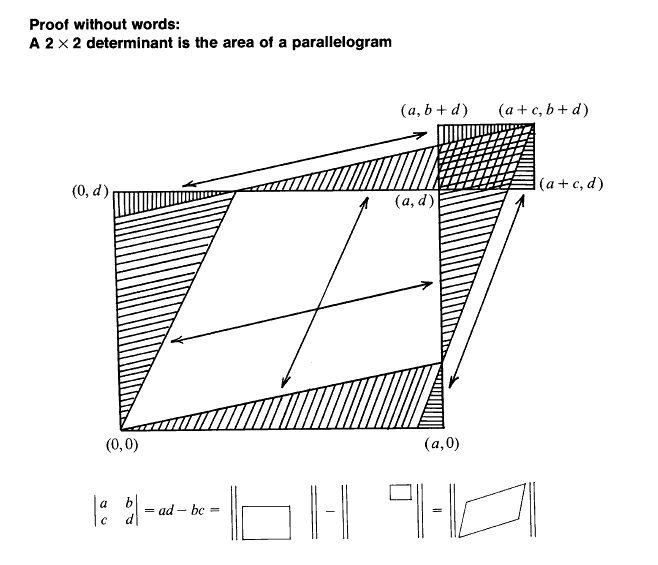
\includegraphics[scale=0.5]{images/2x2detproof.png}
    \caption{A Proof without Words, by Solomon W. Golomb (Mathematics Magazine, March 1985)}
\end{figure}

Observe that the figure above shows that \begin{equation*}
        \Big|\textnormal{det}\begin{bmatrix}
a & b \\
c & d
\end{bmatrix}\Big| = \textnormal{area}(P)
    \end{equation*}
    
       That is, the absolute value of a $2 \times 2$
determinant equals the area of the parallelograms spanned by the rows.  

In other words, the determinant of a $2 \times 2$ matrix $A$ measures the area of the parallelogram spanned by $A\bm{e_1} = \langle a, c \rangle $ and $A\bm{e_2} = \langle b, d \rangle$.   That is, it measures the area of the image of the unit square under the linear transformation $T: \R^2 \to \R^2$ defined by $T(\bm{v}) = A\bm{v}$.

\begin{motivating}
Does this generalize to linear transformations in higher dimensions?
\end{motivating}

\begin{definition}
    
Given three vectors $\bm{u}$, $\bm{v}$, and $\bm{w}$ in $\R^3$, they span a \textbf{parallelpiped}\define{parallelpiped}.  That is, a 3-dimensional solid, such that each face is a parallelogram.

\begin{center}
    
    \begin{tikzpicture}[scale=.7]
    \newcommand{\Depth}{3}
    \newcommand{\Height}{2.5}
    \newcommand{\Width}{4}
    \newcommand{\Skew}{1}

    \coordinate (a) at (0,0,0);
    \coordinate (b) at (\Width,0,0);
    \coordinate (c) at (\Width + \Skew,\Height,\Skew);
    \coordinate (d) at (\Skew,\Height,\Skew);
    \coordinate (e) at (0,0,\Depth);
    \coordinate (f) at (\Width,0,\Depth);
    \coordinate (g) at (\Width + \Skew,\Height,\Depth + \Skew);
    \coordinate (h) at (\Skew,\Height,\Depth + \Skew);

    \coordinate (i) at (\Skew,5,\Depth+ 2.5);

    \draw[fill=rosequartz!30,opacity=0.6] (a) -- (b) -- (c) -- (d) -- (a);
    \draw[fill=rosequartz!30,opacity=0.6] (a) -- (e) -- (f) -- (b) -- (a);
    \draw[fill=rosequartz!30,opacity=0.6] (a) -- (d) -- (h) -- (e) -- (a);
    \draw[fill=rosequartz!30,opacity=0.6] (d) -- (c) -- (g) -- (h) -- (d);
    \draw[fill=rosequartz!30,opacity=0.6] (e) -- (f) -- (g) -- (h) -- (e);
    \draw[fill=rosequartz!30,opacity=0.6] (b) -- (c) -- (g) -- (f) -- (b);
    
    \draw[red, thick, -Latex] (e) -- (h) node[midway,right] {$\bm{u}$};
    \draw[megreen, thick, -Latex] (e) -- (a) node[midway,right] {$\bm{v}$};
    \draw[UCLAblue, thick, -Latex] (e) -- (f) node[midway, below left] {$\bm{w}$};
    
    \draw[dashed, -Latex] (e) -- (i) node[midway, left] {$\bm{v \times w}$};
    
    % \node[place, label=below right:{(4,2,1)}] at (a) {};
    % \node[place, label=right:{(1,7,1)}] at (b) {};
    % \node[place, label=above:{(2,9,7)}] at (c) {};
    % \node[place, label=above:{(5,4,7)}] at (d) {};
    % \node[place, label=below:{(8,1,0)}] at (e) {};
    % \node[place, label=below:{(5,6,0)}] at (f) {};
    % \node[place, label=above left:{(6,8,6)}] at (g) {};
    % \node[place, label=left:{(9,3,6)}]  at (h) {};

\end{tikzpicture}
    
\end{center}
\end{definition}

We can again use geometry to compute the volume of this parallelpiped:

\begin{theorem}
    Let $D$ be the parallelpiped spanned by $\bm{u}$, $\bm{v}$, and $\bm{w}$, and let $\theta$ be the angle between $\bm{u}$ and $\bm{v \times w}$. Then $$\textnormal{volume}(D) = ||\bm{v \times w}|| \ ||\bm{u}|| \ |\cos(\theta)|$$
    \end{theorem}

Observe that we can write this formula in terms of a dot product.

\begin{definition}
        The scalar $\bm{u} \cdot (\bm{v \times w})$ is called the \textbf{scalar triple product}\define{scalar triple product}.
\end{definition}

\begin{example}
Let $D$ be the parallelpiped spanned by $\bm{u} = \langle 1, 3, 2 \rangle$, $\bm{v} = \langle 6, 5, 4 \rangle$, and $\bm{w} = \langle 2, 2, 2 \rangle$.  Compute the volume of $D$.

\end{example}

This computation should seem familiar to you: see example \ref{det3d}

\begin{theorem}
    Let $D$ be the parallelpiped spanned by $\bm{u} = \langle u_1, u_2, u_3 \rangle$, $\bm{v} = \langle v_1, v_2, v_3 \rangle$, and $\bm{w} = \langle w_1, w_2, w_3 \rangle$.  Then
    \begin{equation*}
\textnormal{volume}(D) = |\bm{u} \cdot (\bm{v \times w})| = | \textnormal{det}
\begin{bmatrix}
\bm{u} \\
\bm{v} \\
\bm{w} \\
\end{bmatrix}|
\end{equation*}

    \end{theorem}


\begin{example}
    \begin{definition}
        We say that three vectors $\bm{u}, \bm{v}, \bm{w} \in \R^n$ are \textbf{co-planar}\define{co-planar} if they all lie in the same plane. 
    \end{definition}
    
    Show that if $\bm{u}, \bm{v}, \bm{w} \in \R^3$ are co-planar, then $\textnormal{volume}(D) = 0$.  What is the geometric interpretation of this fact?
\end{example}

Just as we saw in the $2 \times 2$ case, we see again that the determinant of a $3 \times 3$ matrix $A$ measures the volume of the parallelpiped spanned by $A\bm{e_1}$, $A\bm{e_2}$, and $A\bm{e_3}$.  That is, it measures the volume of the image of the unit cube under the linear transformation $T: \R^2 \to \R^2$ defined by $T(\bm{v}) = A\bm{v}$.

This generalizes to $n \times n$ matrices and their associated linear transformations $T:\R^n\to \R^n$.  The determinant will measure the $n$-dimensional volume of the $n$-dimensional parallelpiped spanned by the image of the unit $n$-cube.  In other words, the absolute value of $\textnormal{det}A$ is the factor by which $T$ magnifies volume; and $\textnormal{det}A$ is zero if and only if T is not invertible. 



    \begin{quote}
        ``The determinant is astonishing."       --- Jerry Shurman, \textnormal{Calculus and Analysis in Euclidean Space}.
    \end{quote}








\subsection{Inner products}

\begin{motivating}
How can we generalize the dot product in  $\R^n$ to an arbitrary vector space $V$?  
\end{motivating}

For $\R^n$, we saw that the dot product satisfies the property $\bm{v} \cdot \bm{v} = ||\bm{v}||^2$. Thus, our generalization should allow us to define a notion of \underline{distance} in an abstract vector space.

\begin{definition}
    
    Given two vectors $\bm{u},\bm{v} \in V$, an \textbf{inner product}\define{inner product} on $V$ is a map $\langle - , - \rangle :  V \times V \to \R$ that is:
    \vspace{1em}
    
    \begin{enumerate}
        \item $\langle \bm{u}, \bm{v} \rangle = \langle \bm{v}, \bm{u} \rangle$ (symmetric).
        \item $\langle - , - \rangle$ is bilinear.
        \item $\langle \bm{v}, \bm{v} \rangle \geq 0$, with equality only when $\bm{v} = \bm{0}$. (positive definite).  
    \end{enumerate}
    
    \end{definition}

\begin{definition}
    Given an innner product$\langle - , - \rangle$ on $V$, the \textbf{norm} (or \textbf{modulus}) of a vector $\bm{v} \in V$ is defined as $$||\bm{v}|| = \sqrt{\langle \bm{v}, \bm{v}\rangle}$$
    \end{definition}
    

\begin{example}
    Given two vectors $\bm{u} = \langle u_1, \cdots, u_n \rangle$ and $\bm{v}  = \langle v_1 , \cdots, v_n \rangle$ in $\R^n$, their \textbf{dot product} is an inner product. $$\bm{u} \cdot \bm{v} = \sum u_iv_i$$
    \end{example}

\begin{theorem}[Properties of an inner product]
    
    \begin{enumerate}
        \item Cauchy-Schwarz inequality: $| \langle \bm{u},\bm{v} \rangle | \leq  | \bm{u}| \ | \bm{v} |$
        \item Triangle inequality: $| \bm{u}+ \bm{v} | \leq  | \bm{u}| +| \bm{v} |$
    \end{enumerate}
    
    \end{theorem}





\begin{motivating}
What is the geometric interpretation of the inner product for an arbitrary vector space?
\end{motivating}

\begin{definition}
    A subset $S = \{\bm{v_1}, \bm{v_2}, \cdots, \bm{v_k}\} \subseteq V$ is said to be \textbf{orthogonal} if $\langle \bm{v_i}, \bm{v_j} \rangle = 0$ for all $i \neq j$.
    
    \vspace{1em}
    
    Furthermore, if $|\bm{v_i}| = 1$ for all $1 \leq i \leq k$, we say that the subset $S = \{\bm{v_1}, \bm{v_2}, \cdots, \bm{v_k}\} \subseteq V$ is \textbf{orthonormal}.
\end{definition}
    
    \begin{proposition}
        Equivalently, a set subset $S = \{\bm{v_1}, \bm{v_2}, \cdots, \bm{v_k}\} \subseteq V$ is orthonormal if $$\langle \bm{v_i}, \bm{v_j} \rangle = \delta_{ij}$$ 
        where $\delta_{ij}$ is the \textbf{Kronecker delta}, which is the symbol $$\delta_{ij} = \left\{
		\begin{array}{ll}
			1 & \text{ if } i = j \\
			0 & \text{ if } i \neq j
		\end{array}
		\right.$$
    \end{proposition}


\subsection{Exercises}

\begin{problem}{orthogonal1}
     Find all values of $b$ such that the vectors $\bm{u} = \langle b,3,2\rangle$ and $\bm{v} = \langle 1,b,1\rangle$ are orthogonal.
\end{problem}

\begin{problem}{axiomcalc}
    Given that $||\bm{u}|| = 1$, $||\bm{v}|| = 3$, and $\bm{u} \cdot \bm{v} = 2$, evaluate the expression $2\bm{u} \cdot (3\bm{u} - \bm{v})$.
\end{problem}

\begin{problem}{axiomcalc2}
    Given that $||\bm{u}|| = 2$, $||\bm{v}|| = 3$, and the angle between $\bm{u}$ and $\bm{v}$ is $120^\circ$, calculate $||3\bm{u}-\bm{v}||^2$.
\end{problem}

\begin{problem}{triangle}
    Consider the points $P= (0,8,3)$, $Q= (1,3,0)$, and $R= (1,5,-2)$.   Does the triangle $PQR$ have (A) an obtuse angle (and two acute angles); (B) a right angle (and two acute angles); or (C) three acute angles?
\end{problem}

\begin{problem}{projection}
    Consider the points $P= (0,8,3)$, $Q= (1,3,0)$, and $R= (1,5,-2)$, find the projection of $\bm{PQ}$ in the direction of $\bm{PR}$.
\end{problem}

\begin{problem}{projection2}
    Find the projection of $\bm{u} = \langle 5,7,-4\rangle$ along $\bm{v} = \langle0,0,1\rangle$.
\end{problem}

\begin{problem}{projection3}
    Find the projection of $\bm{u} = \langle a,a,b\rangle$ along $\bm{v} = \bm{i} - \bm{j}$.
\end{problem}

\begin{problem}{projection4}
    Given $\bm{u} = \langle 4, -1, 2 \rangle$, and $\bm{v} = \langle 1, 0, 1 \rangle$
    
    \begin{subproblems}
    \item Find the vectors $\bm{u}_{||\bm{v}}$ and $\bm{u}_{\bot\bm{v}}$
    \item Find the vectors $\bm{v}_{||\bm{u}}$ and $\bm{v}_{\bot\bm{u}}$
    \end{subproblems}
    
\end{problem}


\begin{problem}{plane}
    Write the equation of the plane in $\R^3$ with normal vector $\bm{n} = \langle-1,2,1\rangle$ passing through the point $(4,1,5)$.
\end{problem}

\begin{problem}{plane2}
    Find the equation of the plane in $\R^3$  passing through the points $P = (5,1,1)$, $Q = (1,1,2)$, $R = (2,1,1)$.
\end{problem}

\begin{problem}{plane3}
    Find the equation of the plane in $\R^3$ that contains the lines $$\bm{r_1}(t)= \langle 2 + t, 2 + 3t, 3+ t \rangle$$ $$\bm{r_2}(s)= \langle 5 + s, 15 + 4s, 10 + 2s \rangle$$
\end{problem}

\begin{problem}{plane4}
    Consider the plane $P$ in $\R^3$ given by the equation $3x + 5y-2z = 29$. Find the equation of the plane $R$ that is parallel to $P$ and passes through the point $(3,-1,1)$.
\end{problem}


\begin{definition}
    Let $A$ be a nonempty subset of an inner product space $V$.  The \textbf{orthogonal complement} of $A$ is the subspace
    $$A^\bot := \{\bm{v} \in V \ | \ \langle \bm{a}, \bm{v} \rangle = 0 \ \text{for every } \bm{a} \in A \}$$
    \end{definition}

\begin{problem}{Subspacenk}
    
    
    Prove that $A^\bot$ is a vector subspace.  
    
    
    Let $A = \{\bm{u_1}, \cdots \bm{u_k}\}$ be $k$ linearly independent vectors in a vector space $V$ of dimension $n$. Prove that $A^\bot$ is a subspace of dimension $n-k$.
    
    Describe $A^\bot$ is the intersection of $k$ hyperplanes.
    
\end{problem}

\begin{problem}{crossprodcalc}
    Calculate the cross product of $\bm{u} = \langle 1,1,0\rangle$ and $\bm{v} = \langle 0,1,1\rangle$
\end{problem}

\begin{problem}{parallelogram}
    Consider the points $P= (0,8,3)$, $Q= (1,3,0)$, and $R= (1,5,-2)$, find the area of the parallelogram spanned by   $\bm{PQ}$ and  $\bm{PR}$.
\end{problem}

\begin{problem}{parallelogram2}
    Find the area of the parallelogram determined by the vectors $\langle a, 0, 0\rangle$ and $\langle 0, b, c\rangle$
\end{problem}

\begin{problem}{trianglecross}
    Consider the points $P= (0,8,3)$, $Q= (1,3,0)$, and $R= (1,5,-2)$, find the area of the triangle spanned by   $\bm{PQ}$ and  $\bm{PR}$.
\end{problem}

\begin{problem}{parallelpiped1}
    Consider the points $P= (-1,8,3)$, $Q= (2,3,0)$, $R= (2,5,-2)$, and $S = (3,5,2)$. Find the volume of the parallelpiped that has vertices $P$, $Q$, $R$, and $S$.
    
\end{problem}

\begin{problem}{parallelpiped2}
    Find the volume of the parallelpiped in $\R^3$ spanned by the vectors $\bm{u} =\langle 1, 0,4 \rangle$, $\bm{v} = \langle 1, 3, 1 \rangle$, $\bm{w} = \langle -4, 2, 6 \rangle$.
\end{problem}

\begin{problem}{parallelpiped3}
    Let $P$ be the parallelpiped contained in the first octant (that is, all points in $P$ satisfy $x \geq 0$, $y \geq 0$, $z \geq 0$) determined by the vertices $A= (2,4,1)$, $B= (5,2,5)$, $C= (1,2,4)$, and $D = (1,1,1)$. Find the point $X$ in the parallelpiped $P$ that is \textbf{furthest} from the origin. (\textbf{Hint:} Draw a picture).
\end{problem}

\begin{problem}{lineorplane}
    Do the points $P = (0,1,1)$, $Q = (1,1,2)$, $R = (3,3,3)$ determine a plane or a line?  Find the equation of either the plane or the line.
\end{problem}

\begin{problem}{planesandlines}
    Let $P$ be the plane given by the equation $-3x - 4y+2z = -10$. The plane $P$ intersects the plane $z=0$ at some \textbf{acute} angle $\theta$.  Determine the value of $\cos(\theta)$.
\end{problem}

\begin{problem}{lineplane}
    The intersection of the plane $-3x - 4y+2z = -10$ and the plane $z=0$ is a line $L$.  Find a vector parametrization of the line $L$.
\end{problem}

\begin{problem}{lineintersect}
    The line $\bm{r}(t) = \langle 2, 2, 8 \rangle + t\langle 0,1,2\rangle$ intersects the sphere $x^2 + (y+3)^2 + (z+2)^2 = 9$ in two points.  Find these two points.
\end{problem}